\documentclass[11pt, final]{article}
\usepackage{mystyle}

\addbibresource{./references.bib}

\declaretheorem{definition}
\declaretheorem{example}
\declaretheorem{theorem}
\declaretheorem{lemma}
\declaretheorem{corrollary}
\renewcommand{\headrulewidth}{0.5pt}
\renewcommand{\footrulewidth}{0.5pt}
\renewcommand{\listingscaption}{Code snippet}
\newenvironment{subproof}[1][\proofname]{%
  \renewcommand{\qedsymbol}{$\blacksquare$}%
  \begin{proof}[#1]%
}{%
  \end{proof}%
}
\newenvironment{llisting}{\captionsetup{type=listing}}{}

% lang
\newcommand{\var}[1]{\texttt{var}\ #1}
\newcommand{\rval}[1]{\texttt{rval}\ #1}
\newcommand{\abs}[1]{\texttt{abs}\ #1}
\newcommand{\first}[1]{\texttt{first}\ #1}
\newcommand{\second}[1]{\texttt{second}\ #1}
\newcommand{\add}[2]{\texttt{add}\ #1\ #2}
\newcommand{\build}[2]{\texttt{build}\ #1\ #2}
\newcommand{\get}[2]{\texttt{get}\ #1\ #2}
\newcommand{\mul}[2]{\texttt{mul}\ #1\ #2}
\newcommand{\app}[2]{\texttt{app}\ #1\ #2}
\newcommand{\tuple}[2]{\texttt{tuple}\ #1\ #2}
\newcommand{\case}[3]{\texttt{case}\ #1\ #2\ #3}
\newcommand{\inl}[1]{\texttt{inl}\ #1}
\newcommand{\inr}[1]{\texttt{inr}\ #1}
\newcommand{\nval}[1]{\texttt{nval}\ #1}
\renewcommand{\nsucc}[1]{\texttt{nsucc}\ #1}
\newcommand{\nrec}[3]{\texttt{nrec}\ #1\ #2\ #3}

\newcommand{\tm}[2]{tm\ #1\ #2}
\newcommand{\Fin}[1]{Fin\ #1}
\newcommand{\Array}[2]{Array\ #1\ #2}

\newcommand{\denR}[0]{\mathcal{R}}
\newcommand{\denN}[0]{\mathcal{N}}

% Keywords and shortcuts
\newcommand{\Coq}[0]{\textbf{Coq}}

% Syntactic terms
\def\Vakar{V\'{a}k\'{a}r}
\def\D{\overrightarrow{\mathcal{D}}}
\def\lambdaBase{\Lambda_{\delta}^{\times, \rightarrow, \mathds{R}}}
\def\<#1>{\csname keyword@@#1\endcsname}
\begingroup
\makeatletter
\def\do#1{\expandafter\doaux\expandafter{\keyword@style{#1}}{#1}}
\def\doaux#1#2{\global\@namedef{keyword@@#2}{#1}}
\def\keyword@style#1{\textit{#1}}
\do{Coq}
\do{Agda}
\def\keyword@style#1{\texttt{#1}}
\do{R}
\do{N}
\do{bottom}
\do{Equations}
\do{Coquelicot}
\do{Program}
\do{Set}
\do{Prop}
\do{Type}
\do{return}
\do{simpl}
\do{Either}
\do{Fin}
\do{Reals}
\do{var}
\do{abs}
\do{app}
\do{tuple}
\do{first}
\do{second}
\do{rval}
\do{add}
\do{mul}
\do{nval}
\do{nsucc}
\do{nrec}
\do{case}
\do{inl}
\do{inr}
\do{build}
\do{get}
\do{Top}
\do{Pop}
\do{hd}
\do{tl}
\endgroup


\setlength{\headheight}{15pt}
\pagestyle{fancy}
\lhead{Utrecht University}
\rfoot{\thepage}
\cfoot{ }
\allowdisplaybreaks

\begin{document}

\begin{titlepage}
  \pagenumbering{gobble}

  \begin{figure}
    \begin{minipage}{0.48\textwidth}
    \begin{flushleft}
    %  \includegraphics[scale=0.5]{Images/UU_LOGO.png}
    \end{flushleft}
    \end{minipage}\hfill
    \begin{minipage}{0.48\textwidth}
    \begin{flushright}
    %  \includegraphics[scale=0.2]{Images/Logo.png}
    \end{flushright}
    \end{minipage}
  \end{figure}

  \thispagestyle{fancy}

  \vspace{1in}

  \center

  \textsc{\large Master Thesis}

  \vspace{0.5in}

  \noindent\makebox[\linewidth]{\rule{\linewidth}{1.2pt}}
  \textsc{\textbf{\large Formalized Correctness Proofs of Automatic Differentiation in Coq}}
  \noindent\makebox[\linewidth]{\rule{\linewidth}{1.2pt}}

  \vspace{0.5in}

  \begin{minipage}{0.48\textwidth}
    \begin{flushleft}
      \textit{Student:} \\
      Curtis Chin Jen Sem \\
      \textit{5601118}
      % crtschin@gmail.com
    \end{flushleft}
  \end{minipage}
  \begin{minipage}{0.48\textwidth}
    \begin{flushright}
    \textit{Supervisors:} \\
    Matthijs \Vakar \\
    Wouter Swierstra \\
    \end{flushright}
  \end{minipage}

  \vspace{2in}

  \textbf{\large Department of Information and Computing Science} \\
  % \textit{Last updated: \today}
\end{titlepage}

\newpage

\begin{abstract}
  Automatic differentiation is a well-known concept, which has been gaining traction is recent years due to its heavy usage in many versatile applications.
  Exposing the decades-worth of programming language history to this technique may bear fruit with improving both performance, correctness and modularity of such code.
  While pen-and-paper proofs of correctness do exist for these techniques in the context of functional languages, a formal proof has been absent up till now.
  In this research, we give a formalized proof of correctness of both a ubiquitous forward-mode and a continuation-based psuedo reverse-mode automatic differentiation algorithms.
  We repeatedly do this using a logical relations argument accompanied with simple but effective language representations and denotations.
  We also discuss and prove sound various program transformations, which lets forward-mode automatic differentiation approach the performance of reverse-mode.
  We also make preliminary steps towards a formalized proof of correctness of a real combinator-based reverse-mode algorithm.
\end{abstract}

\newpage

\pagenumbering{arabic}
\setcounter{page}{3}
\tableofcontents
\newpage

\section{Introduction}
% TODO: Work through MV feedback
Automatic differentiation is a well-known technique within the scientific community with diverse applications such as Bayesian inference and solving systems of non-linear algebraic equations.
It has received increased interest due to recent developments in machine learning research, where solving optimization problems is the primary goal.
One of the algorithms involved in this area of research is known as backpropagation.
Backpropagation directly corresponds to reverse-mode automatic differentiation, which, in most cases, is the most efficient method to compute the derivatives of a function, critical in optimization problems.
However, programming in an environment that allows for automatic differentiation can be limiting.

Frameworks such as Tangent\fancyfootnote{https://github.com/google/tangent} or autograd\fancyfootnote{https://github.com/HIPS/autograd} are define-by-run algorithms, whose main tactic is to build up the derivative calculation dynamically during runtime.
This process can restrict which high-level optimizations one can apply to generated code.
Support for higher-order derivatives is also limited.

Programming language research has a rich history, with many well-known both high and low-level optimization techniques such as partial evaluation and deforestation.
Exposing these optimization techniques to the world of automatic differentiation can be very fruitful as these calculations are costly and often require significant computing power to run.
Through other concepts such as higher-order functions and type systems, we would also get additional benefits such as code-reusability and correctness.

While much research has already been done to integrate programming language theory with automatic differentiation, formalizations of these techniques are absent.
In this thesis, we aim to formalize an extensible correctness proofs of various implementations of automatic differentiation on a simply-typed lambda calculus in the \<Coq> proof assistant, opening up further possibilities for formally proving the correctness of more complex language features in the future.
Our formalization is based on a recent proof by Huot, Staton, and \Vakar{} \cite{huot2020correctness}.
They proved, using a denotational model of diffeological spaces, that their forward-mode emulating macro is correct when applied to a simply-typed lambda calculus with products, co-products and inductive types.

With this thesis we make the following core contributions:
\begin{itemize}
  \item Formalize the proofs of both the forward-mode and continuation-based automatic differentiation algorithms specified by Huot, Staton, and \Vakar{} \cite{huot2020correctness} in \<Coq>.
  \item Prove the semantic correctness of various useful compile-time optimizations techniques in the context of generating performant code for automatic differentiation.
  \item Extend the proofs with the array types and compile-time optimization rules by Shaikhha et al.\cite{Shaikha2019}.
  \item Analyze both the requirements of and issues involved with giving a formal proof of correctness for the combinator-based reverse-mode automatic differentiation algorithm by \Vakar{}\cite{vkr2020reverse}.
\end{itemize}

\Cref{sec:bg} includes a background section explaining many of the topics and techniques used in this thesis. The formalization of the ubiquitous forward-mode automatic differentiation is given in \cref{sec:forward}, starting from a base simply-typed lambda calculus extended with product types and incrementally adding new types and language constructs. \Cref{sec:opt,sec:continuation-base} give formalizations of optimization avenues through, respectively, program transformations and a continuation-based automatic differentiation algorithms.
Finally, \cref{sec:rev} gives our attempt at a formal proof of the combinator-based reverse-mode automatic differentiation algorithm.
The proofs resulting from the development of this work is available in an online repository\cite{curtis_chin_jen_sem_2020_4022908}.

As a notational convention, we will use specialized notation in the definitions themselves.
\<Coq> normally requires that pretty printed notations be defined separately from the definitions they reference.


\section{Background}
\subsection{Automatic differentiation}
Automatic differentiation (\textit{AD}) has a long and rich history, where its driving motivation is to efficiently calculate the derivatives of functions in a manner that is both correct and fast\cite{Baydin2015AutomaticDI}.
There are several different methods of implementing AD algorithms, such as source-code transformations or operator overloading.
These algorithms usually transform any program which implements some function to one that calculates its derivative.

There are two main variants of AD, namely forward-mode and reverse-mode AD.
In forward-mode AD, every term in the function trace is annotated with the corresponding derivative of that term.
These are also known as the respectively the primal and tangent traces.
So calculating the partial derivatives of sub-terms is structure preserving with respect to the normal calculation of terms.

This approach to forward-mode AD can be explained by dual numbers as these are, mathematically seen, what we are calculating with\cite{Baydin2015AutomaticDI}. Dual numbers are numbers of the form of
$$
  x + x' \epsilon
$$
where $x, x' \in \denR$ and $\epsilon$ is a nilpotent number, such that $\epsilon^2 = 0$ and $\epsilon \neq 0$.
Notably, both primal and tangent values are tracked in this representation, namely the tangent value is present in the coefficients of $\epsilon$.
As an example, we can see that this is true for both addition and multiplication:
\begin{align*}
  (x + x' \epsilon) + (y + y' \epsilon) &= (x + y) + (x' + y')\epsilon \\
  (x + x' \epsilon)(y + y' \epsilon) &= (xy) + (xy' + yx')\epsilon
\end{align*}
Using the following scheme for function application:
\begin{align*}
  f(x + x' \epsilon) &= f(x) + f'(x)x'\epsilon
\end{align*}
We can also see that it follows the chain rule for function composition.
\begin{align*}
  f(g(x + x' \epsilon)) &= f(g(x) + g'(x)x'\epsilon)) \\
    &= f(g(x)) + f'(g(x))g'(x)x'\epsilon
\end{align*}
Using this, we can essentially calculate the derivative of any derivable function by interpreting any non-dual number $x$ as its dual number counterpart of either $x + 1\epsilon$ or $x + 0\epsilon$. We interpret constant values as $x + 0\epsilon$, while input variables we take the partial derivative of are interpreted as $x + 1\epsilon$.

To give a more elaborate example of how this works in forward-mode AD, take the function $f(x, y) = x^2 + (x - y)$ as an example.
The dependencies between the terms and operations of the function is visible in the computational graph in \cref{fig:func_trace}.
The corresponding traces are filled in \cref{table:func_trace} for the input values $x = 2, y = 1$.
We can calculate the partial derivative $\frac{\delta f}{\delta x}$ at this point by setting $x' = 1$ and $y' = 0$.
Note that the calculation of the traces is structural.
When calculating the primal value at a specific point, we can calculate the corresponding tangent value at that same point.

\begin{figure}
  \centering
  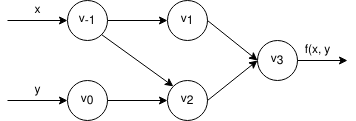
\includegraphics[scale=0.6]{./assets/function_trace.png}
  \caption{Computational graph of $f(x, y) = x^2 + (x - y)$}
  \label{fig:func_trace}
\end{figure}

\begin{table}
  \begin{center}
    \begin{tabular}{ l l l l l | l l l l l }
      \hline
      \multicolumn{5}{l}{Primal trace} & \multicolumn{5}{l}{Tangent trace} \\
      \hline
$v_{-1} $&$=$&$x$&$=$&$2$             &$v'_{-1}$&$=$&$x'$&$=$&$1$ \\
$v_0    $&$=$&$y$&$=$&$1$             &$v'_{0}$&$=$&$y'$&$=$&$0$ \\
      \hline
$v_1    $&$=$&$v_{-1}^2$&$=$&$4$      &$v'_{1}$&$=$&$2*v_{-1}$&$=$&$4$ \\
$v_2    $&$=$&$v_{-1} - v_{0}$&$=$&$1$&$v'_{2}$&$=$&$v'_{-1}-v'_{0}$&$=$&$1$ \\
$v_3    $&$=$&$v_1 + v_2$&$=$&$5$     &$v'_{3}$&$=$&$v'_1 + v'_2$&$=$&$5$ \\
      \hline
$f      $&$=$&$v_3$&$=$&$5$           &$f'$&$=$&$v'_3$&$=$&$5$ \\
      \hline
    \end{tabular}
  \end{center}
  \caption{Primal and tangent traces of $f(x, y) = x^2 + (x - y)$}
  \label{table:func_trace}
\end{table}

Reverse-mode automatic differentiation takes a drastically different approach.
It starts by annotating one of the possibly many output variables $\frac{\partial{y}}{\partial{y}} = 1$ and working in the reverse direction, annotating each intermediate variable $v_i$ with their adjoint
$$v'_i=\frac{\delta y_i}{\delta v_i}$$
To accomplish this, two passes are necessary.
Like the forward-mode variant, a primal trace is needed.
This first pass functions to determine the intermediate variables and their respective dependencies.
The second pass in the algorithm calculates the partial-derivatives by working backwards from the output using the adjoints, also called the adjoint trace.
When variables are used multiple times, also called fan-out, their adjoints are added in the adjoint trace.
% TODO: Mention something about define-then-run/define-by-run and how they work with regards to strategy.
% Tape recording using operator overloading/specialized semantics

The optimal choice between automatic differentiation variant is heavily dependent on the specific function being differentiated.
Preference is given for forward-mode AD when the number of output variables exceeds the number of input variables, as it has to be rerun for each partial derivative of the function.
On the other hand, as reverse-mode AD works backwards, the reverse-pass needs to be redone for each output variable.
In machine learning research, reverse-mode AD is generally preferred as the objective functions generally contain a small number of output variables.

% TODO: Mention something about Eliott's categorical approach and its possible extension to a macro on combinators.

\subsection{Denotational semantics}
% A formal semantics of programming language: An introduction
% TODO: Work through MV feedback
Denotational semantics enables reasoning about programs using formal mathematics.
It also functions as a hotbed for new and innovative language designs and algorithms.
The most well-known example is the domain theory model given by Dana Scott and Christopher Strachey\cite{Scott1977} for lambda calculi.
To be able to formalize non-termination and partiality, they thought to use concepts such as partial orderings and least fixed points\cite{aaby2020}.
In this model, programs are regularly interpreted as partial functions, and recursive computations as taking the fixpoint of such functions.
Non-termination, on the other hand, is formalized as a value $\bot$ that is lower in the ordering relation than any other element.

Automatic differentiation introduces a challenge in constructing a denotational semantics as the notion of differentiability needs to be included.
If the language under consideration were to be restricted to real-typed terms, Cartesian spaces would have been sufficient as any well-typed term $x_1 : \synR, \dots, x_n : \synR \vdash t : \synR$ could be interpreted as the corresponding smooth function $\llbracket t \rrbracket : \denR^n \to \denR$.
Note that we use $\synR$ as the syntactic type for real numbers, while $\denR$ is its denotational counterpart.
Using Cartesian spaces, however, does not work when function types are added as their denotational equivalent, function spaces, are not supported\cite{huot2020correctness}.
The original pen and paper proof of automatic differentiation this thesis is based on by Huot, Staton and \Vakar{}\cite{huot2020correctness}, remedies this issue by using diffeological spaces as the underlying mathematical model.

For the purpose of this thesis, however, we were able to avoid using diffeological spaces by directly encoding the property of differentiability in the logical relation itself.
We were also able to avoid domain theoretical models such as $\omega$-cpos by excluding language constructs such as recursion and iteration where non-termination and partiality come into play.
As a part of its type system, \<Coq> contains a set-theoretical model available under the sort \<Set> in its type system, which is satisfactory as the denotational semantics for our language.

Because we use real numbers as the ground type in our language, we also needed an encoding of the real numbers in \<Coq>.
While support for real numbers in the standard library in \<Coq> has improved in recent times from one based on an axiomatic definition to one involving Cauchy sequences\fancyfootnote{https://coq.inria.fr/library/Coq.Reals.ConstructiveCauchyReals.html}, it is still insufficient for our purposes.
We also need a notion of differentiability which we will use to among others, phrase correctness of our automatic differentiation macros.
Instead of attempting to encode this by hand, we opted for the more comprehensive library \<Coquelicot>\cite{Boldo2015CoquelicotAU}, which contains many useful user-friendly definitions for doing calculus.

\subsection{Coq}
% TODO: Work through MV feedback
\<Coq> is a proof assistant based on the calculus of constructions type theory created by Thierry Coquand and G\'{e}rard Huet\cite{Coquand1988}.
In the past 30 years since it has been released, research has contributed to extending the proof assistant with additional features such as inductive and co-inductive data types\cite{Coquand1990}, dependent pattern matching\cite{Sozeau2010} and advanced modular constructions for organizing large mathematical proofs\cite{Sozeau2008}\cite{Mahboubi2013}.

The core of this type theory is based on constructive logic and so many of the laws known in classical logic are not provable.
An example includes the law of the excluded middle, $\forall A, A \vee \neg A$.
In most cases they can, however, be safely added to \<Coq> without making its logic inconsistent. Many of these axioms are readily available in the standard library.
Due to its usefulness in proving propositions over functions, we will make heavy use of the functional extensionality axiom in \<Coq>, which states that functions are equal if they are extensionally equivalent, $(\forall x, f\ x = g\ x) \to f = g$.

\subsubsection{Language representation}
\label{sec:language_repr}

\begin{figure}
  \begin{mathpar}
    \inferrule*[Right=\textsc{TVar}]
      {elem\ n\ \Gamma = \tau}
      {\Gamma \vdash var\ n : \tau} \and
    \inferrule*[Right=\textsc{TAbs}]
      {(\sigma, \Gamma) \vdash t : \tau}
      {\Gamma \vdash t : \sigma \rightarrow \tau} \\ \and
    \inferrule*[Right=\textsc{TApp}]
      {\Gamma \vdash t1 : \sigma \rightarrow \tau \\
        \Gamma \vdash t2 : \sigma}
      {\Gamma \vdash t1\ t2 : \tau}
  \end{mathpar}
  \label{fig:stlc_infer}
  \caption{Type-inferrence rules for a simply-typed lambda calculus using De-Bruijn indices}
\end{figure}

When defining a simply-typed lambda calculus, there are two main possibilities\cite{plfa2019}.
The arguably simpler variant, known as an extrinsic representation, is traditionally the one introduced to new students learning \<Coq>.
In the extrinsic representation, the terms themselves are untyped and typing judgments are defined separately as relations between the types and terms. A basic example of working with this is given in Software Foundations\cite{Pierce:SF2}.
This, however, required many additional lemmas and machinery to be proved to be able to work with both substitutions and contexts as these are defined separate from the terms.
As an example, the preservation property which states that reduction does not change the type of a term, needs to be proven explicitly.
The other approach, also called an intrinsic representation, makes use of just a single well-typed definition.
Ill-typed terms are made impossible by the type checker.
This representation, while beneficial in the proof load, however complicates much of the normal machinery involved in programming language theory.
One example is how one would define operations such as substitutions or weakening.

But even when choosing an intrinsic representation, the problem of variable binding persists.
Much meta-theoretical research has been done on possible approaches to this problem each with their own advantages and disadvantages.
The POPLmark challenge gives a comprehensive overview of each of the possibilities in various proof assistants\cite{Aydemir2005}.
An example of an approach is the nominal representation where every variable is named.
While this does follow the standard format used in regular mathematics, problems such as alpha-conversion and capture-avoidance appears.

\begin{listing}[h]
  \begin{minted}{coq}
  Inductive ty : Type :=
    | ~unit~ : ty
    | ~\Rightarrow~ : ty ~\rightarrow~ ty ~\rightarrow~ ty.

  Inductive tm : Type :=
    | var : string ~\rightarrow~ tm
    | abs : string ~\rightarrow~ ty ~\rightarrow~ tm ~\rightarrow~ tm
    | app : tm ~\rightarrow~ tm ~\rightarrow~ tm.
  \end{minted}
  \caption{Simply typed \lambda-calculus using an extrinsic nominal representation.}
  \label{lst:nominal_stlc}
\end{listing}

The approach used in the rest of this thesis is an extension of the De-Bruijn representation which numbers variables relative to the binding lambda term.
In this representation the variables are referred to as well-typed De-Bruijn indices.
A significant benefit of this representation is that the problems of capture avoidance and alpha equivalence are avoided.
As an alternative, instead of using numbers to represent the distance, indices within the typing context can be used to ensure that a variable is always well-typed and well-scoped.
While the idea of using type indexed terms has been both described and used by many authors\cite{Altenkirch99}\cite{McBride04}\cite{Adams06}, the specific formulation used in this thesis using separate substitutions and rename operations was fleshed out in Coq by Nick Benton, et. al.\cite{Benton2011}, and was also used as one of the examples in the second POPLmark challenge which deals with logical relations\cite{poplmark_reloaded}.
While this does avoid the problems present in the nominal representation, it unfortunately does have some problems of its own.
Variable substitutions have to be defined using two separate renaming and substitution operations.
Renaming is formulated as extending the typing context of variables, while substitution actually swaps the variables for terms.
Due to using indices from the context as variables, some lifting boilerplate is also needed to manipulate contexts.

\begin{listing}[h]
  \begin{minted}{coq}
  Inductive ~\tau \in \Gamma~ : Type :=
    | Top : ~\forall \Gamma \tau, \tau \in (\tau::\Gamma)~
    | Pop : ~\forall \Gamma \tau \sigma, \tau \in \Gamma \rightarrow \tau \in (\sigma::\Gamma)~.

  Inductive tm ~\Gamma \tau~ : Type :=
    | var : ~\forall \Gamma \tau, \tau \in \Gamma \rightarrow tm \Gamma \tau~
    | abs : ~\forall \Gamma \tau \sigma, tm (\sigma::\Gamma) \tau \rightarrow tm \Gamma (\sigma \Rightarrow \tau)~
    | app : ~\forall \Gamma \tau \sigma, tm \Gamma (\sigma \Rightarrow \tau) \rightarrow tm \Gamma \sigma \rightarrow tm \Gamma \tau~.
  \end{minted}
  \caption{Basis of a simply-typed \lambda-calculus using a strongly typed intrinsic formulation.}
  \label{lst:strong_stlc}
\end{listing}

% TODO: Work out how substitutions work

\subsubsection{Dependently-typed programming in Coq}
% TODO: Work through MV feedback
In \<Coq>, one can normally write function definitions using either case-analysis as is done in other functional languages, or using \<Coq>'s tactics language.
Using the standard case-analysis functionality can cause the code to be complicated and verbose, even more so when proof terms are present in the function signature.
This has been caused by the previously poor support in \<Coq> for dependent pattern matching.
Using the return keyword, one is able to vary the result type of a match expression. But due to requirement \<Coq> used to have that case expressions be syntactically total, this could be very difficult to work with.
One other possibility would be to write the function as a relation between its input and output.
This also has its limitations as you then lose computability as \<Coq> treats these definitions opaquely. In this case the standard \<simpl> tactic which invokes \<Coq>'s reduction mechanism is not able to reduce instances of the term.
This often requires the user to write many more proofs to be able to work with the definitions.

As an example, we will work through defining a length indexed list and a corresponding head function limited to lists of length at least one in Snippet~\ref{lst:dt_ilist}.
Using the \<Coq> keyword return, it is possible to let the return type of a match expressions depend on the result of one of the type arguments.
This makes it possible to define an auxiliary function which, while total on the length of the list, has an incorrect return type. It namely returns the type unit if the input list had the length zero.
We can then use this auxiliary function in the actual head function by specifying that the list has length at least one.
It should be noted that more recent versions of \<Coq> do not require that case expressions be syntactically total, so specifying that the input list has a length of at least zero is enough to eliminate the requirement for the zero-case.

\begin{listing}
  \begin{minted}{coq}
  Inductive ilist : ~Type \rightarrow nat \rightarrow Type~ :=
    | nil : ~\forall A, ilist A 0~
    | cons : ~\forall A n, A \rightarrow ilist A n \rightarrow ilist A (S n)~

  Definition hd' {A} n (ls : ilist A n) :=
    match ls in (ilist A n) return
      (match n with
      | O => unit
      | S _ => A end) with
    | nil => tt
    | cons h _ => h
  end.

  Definition hd {A} n (ls : ilist A (S n)) : A := hd' n ls.
  \end{minted}
  \caption{Definition of a length indexed list and hd using the return keyword, adapted from Certified Programming with Dependent Types\cite{ChlipalaCPDT}.}
  \label{lst:dt_ilist}
\end{listing}

Mathieu Sozeau introduces an extension to \<Coq> via a new keyword \<Program> which allows the use of case-analysis in more complex definitions\cite{Sozeau2006}\cite{Sozeau2007}.
To be more specific, it allows definitions to be specified separately from their accompanying proofs, possibly filling them in automatically if possible.
While this does improve on the previous situation, using the definitions in proofs can often be unwieldy due to the amount of boilerplate introduced.
This makes debugging error messages even harder than it already is in a proof assistant. This approach was used by Benton in his formulation of strongly typed terms.

Sozeau further improves on this introducing a method for user-friendlier dependently-typed pattern matching in \<Coq> in the form of the \<Equations> library\cite{Sozeau2010}\cite{Sozeau2019}.
This introduces \<Agda>-like dependent pattern matching with with-clauses.
It does this by using a notion called coverings, where a covering is a set of equations such that the pattern matchings of the type signature are exhaustive.
There are two main ways to integrate this in a dependently typed environment, externally where it is integrated as high-level constructs in the pattern matching core as \<Agda> does it, or internally by using the existing type theory and finding witnesses of the covering to prove the definition correct, which is the approach used by Sozeau.
Due to the intrinsic typeful representation this paper uses, much of this was invaluable when defining the substitution operators as the regular type checker in \<Coq> often had difficulty unifying dependently typed terms in certain cases.

\begin{listing}
  \begin{minted}{coq}
  Equations hd {A n} (ls : ilist A n) (pf : n <> 0) : A :=
  hd nil pf with pf eq_refl := {};
  hd (cons h n) _ := h.
  \end{minted}
  \caption{Definition of hd using \<Equations>}
  \label{lst:dt_ilist_hd_equations}
\end{listing}


\subsection{Logical relations}
% TODO: Work through MV feedback
Logical relations arguments are a proof technique often employed when proving programming language properties of statically typed languages\cite{skorstengaard2019introduction}. There are two main ways they are used, namely as unary and binary relations.
Unary logical relations, also known as logical predicates, are predicates over single terms and are typically used to prove language characteristics such as type safety or strong normalization.
Binary logical relations on the other hand are used to prove program equivalences, usually in the context of denotational semantics as we will do.
There have been many variations on the versatile technique from syntactic step-indexed relations which have been used to reason about recursive types and general references\cite{Ahmed2006}, to open relations which enable working with terms of non-ground type\cite{barthe2020versatility}\cite{huot2020correctness}.
Logical relations in essence are relations between terms defined by induction on their types.
A logical relations proof consists of 2 main steps.
The first states the terms for which the property is expected to hold are in the relation, while the second states that the property of interest follows from the relation.
The second step is easier to prove as it usually follows from the definition of the relation. The first on the other hand, will often require proving a generalized variant, called the fundamental property of the logical relation.
In most cases this requires that the relation is correct with respect to applying substitutions.

A well-known logical relations proof is the proof of strong normalization of well-typed terms, which states that all terms eventually terminate.
An example of a logical relation used in such a proof using the intrinsic strongly-typed formulation is given in Snippet~\ref{lst:sn_logical_relation}.
Noteworthy is the case for function types, where one needs to prove that applying a function preserves the strong normalization property.
If one were to attempt the proof of strong normalization without using logical relations, the proof would get stuck in the cases dealing with function types.
More specifically when applying a function term to an argument term which terminates, the induction hypothesis is not strong enough to prove that substituting the argument into the body of the abstraction results in a terminating term.

% TODO: Remove/Move this
% The proof given in the paper this thesis is based on, is a logical relations proof on the denotational semantics using diffeological spaces as its domains\cite{huot2020correctness}.
% A similar, independent proof of correctness was given by Barthe, et al.\cite{barthe2020versatility} using a syntactic relation on the operational semantics.

\begin{listing}
  \begin{minted}{coq}
    Equations SN {~\Gamma~} ~\tau~ (t : ~tm \Gamma \tau~): Prop :=
    SN unit t := halts t;
    SN ~(\tau \Rightarrow \sigma)~ t := halts t ~$\wedge$~
      ~(\forall (s : tm \Gamma \tau), SN \tau s \rightarrow SN \sigma (app \Gamma \sigma \tau t s))~;
  \end{minted}
  \caption{Example of a logical predicate used in a strong normalization proof in the strongly-typed intrinsic representation}
  \label{lst:sn_logical_relation}
\end{listing}

\subsection{Related work}

% Move this line to related work
% Huot, Staton and \Vakar{} have proposed a continuation-based algorithm which mimic much of the same ideas as reverse mode automatic differentiation\cite{huot2020correctness}.
% \subsection{Notation}

\section{Formalizing Forward-Mode AD}\label{sec:forward}
  We will explain our formalization of the forward-mode automatic differentiation macro in the following sections.
  The formal proof will start from a base simply-typed lambda calculus extended with product types and incrementally add both sum and array types.
  Also included in the final language are natural number types with a primitive recursion principle.
  Many of the theorems and lemmas introduced in \cref{sec:formal_stlc} do not change, as they are independent of the specific types and terms included in the language.
  \subsection{Simply Typed Lambda Calculus}\label{sec:formal_stlc}
  % TODO: Work through MV feedback
  % Talk about simply typed lambda calculus,
  % Something about Λ_δ^{+, *, R}
  % Give examples of functions
  % talk about denotations and
  As mentioned in background section~\ref{sec:language_repr}, we will make use of De-Bruijn indices in a intrinsic representation to formulate our language.
  Both addition and multiplication are included as example operations on the real numbers, but the proofs can be easily extended to other primitive operations.
  Our base language consists of the classic simply-typed lambda calculus with product types and real numbers.

  Both the language constructs and the typing rules for this language are common for a simply typed lambda calculus, as shown in figure~\ref{fig:base_infer}.
  As expected, we include variables, applications and abstractions in the language using, respectively, the \<var>, \<app> and \<abs> constructors.
  We work with projection products, whose elimination rules are encoded in the  \<first> and \<second> constructors. The \<tuple> constructor is used to represent the introduction rule.
  For real numbers, \<rval> is used to introduce real numbered constants and \<add> and \<mul> will be used to respectively encode addition and multiplication.

  \begin{figure}
    \begin{mathpar}
      \inferrule*[Right=\textsc{TVar}]
        {elem\ n\ \Gamma = \tau}
        {\Gamma \vdash \var{n} : \tau} \and
      \inferrule*[Right=\textsc{TAbs}]
        {(\sigma, \Gamma) \vdash t : \tau}
        {\Gamma \vdash \abs{t} : \sigma \rightarrow \tau} \\ \and
      \inferrule*[Right=\textsc{TApp}]
        {\Gamma \vdash t1 : \sigma \rightarrow \tau \\
          \Gamma \vdash t2 : \sigma}
        {\Gamma \vdash \app{t1}{t2} : \tau} \\ \and
      \inferrule*[Right=\textsc{TTuple}]
        {\Gamma \vdash t1 : \tau \\
          \Gamma \vdash t2 : \sigma}
        {\Gamma \vdash \tuple{t1}{t2} : \tau \times \sigma} \\ \and
      \inferrule*[Right=\textsc{TFst}]
        {\Gamma \vdash t : \tau \times \sigma}
        {\Gamma \vdash \first{t} : \tau} \and
      \inferrule*[Right=\textsc{TSnd}]
        {\Gamma \vdash t : \tau \times \sigma}
        {\Gamma \vdash \second{t} : \sigma} \\ \and
      \inferrule*[Right=\textsc{TRVal}]
        {r \in \denoteR}
        {\Gamma \vdash \rval{r} : \<R>} \\ \and
      \inferrule*[Right=\textsc{TAdd}]
        {\Gamma \vdash r1 : \<R> \\
          \Gamma \vdash r2 : \<R> \\ }
        {\Gamma \vdash \add{r1}{r2} : \<R>} \and
      \inferrule*[Right=\textsc{TMull}]
        {\Gamma \vdash r1 : \<R> \\
        \Gamma \vdash r2 : \<R> \\ }
      {\Gamma \vdash \mul{r1}{r2} : \<R>} \and
    \end{mathpar}
    \caption{Type-inference rules for the base simply-typed lambda calculus}
    \label{fig:base_infer}
  \end{figure}

  % How we translated this into the well-typed intrinsic representation
  These can be translated into Coq definitions in a reasonably straightforward manner, with each case keeping track of both how the typing context and types change.
  In the \<var> case we need some way to determine what type the variable is referencing.
  Like many others previously\cite{Benton2011}\cite{Coquand1994}, instead of using indices into the list accompanied with a proof that the index does not exceed the length of the list, we make use of an inductively defined type evidence to type our variables as shown in code snippet~\ref{lst:strong_stlc}.
  The cases for \<app> and \<abs> are as expected, where variables in the body of abstractions are able to reference their respective arguments.

  Note that in the original proof by Huot, Staton, and \Vakar{} \cite{huot2020correctness}, they made use of n-ary products accompanied with pattern matching expressions.
  We opted to implement binary projection products, as these are conceptually simpler while still retaining much of the same functionality expected of product types.

  \begin{minted}{coq}
    Inductive tm ~(\Gamma : Ctx) : ty \rightarrow Type~ :=
      ...
      (* Binary projection products *)
      | tuple : ~forall {\tau \sigma},
        tm \Gamma \tau \rightarrow
        tm \Gamma \sigma \rightarrow
        tm \Gamma (\tau \times \sigma)~
      | first : ~forall {\tau \sigma}, tm \Gamma (\tau \times \sigma) \rightarrow tm \Gamma \tau~
      | second : ~forall {\tau \sigma}, tm \Gamma (\tau \times \sigma) \rightarrow tm \Gamma \sigma~
      (* Operations on reals *)
      | rval : ~forall r, tm \Gamma R~
      | add : ~tm \Gamma R \rightarrow tm \Gamma R \rightarrow tm \Gamma \tau~
      | mul : ~tm \Gamma R \rightarrow tm \Gamma R \rightarrow tm \Gamma \sigma~
  \end{minted}

  % \begin{listing}
  %   \begin{minted}{coq}
  % Definition Ctx : Type := list ty.

  % Inductive tm ~(\Gamma : Ctx) : ty \rightarrow Type~ :=
  %   (* Base STLC *)
  %   | var : ~forall \tau,
  %     \tau ∈ \Gamma \rightarrow tm \Gamma \tau~
  %   | app : ~forall \tau \sigma,
  %     tm \Gamma (\sigma \Rightarrow \tau) \rightarrow
  %     tm \Gamma \sigma \rightarrow
  %     tm \Gamma \tau~
  %   | abs : ~forall \tau \sigma,
  %     tm (\sigma::\Gamma) \tau \rightarrow tm \Gamma (\sigma \Rightarrow \tau)~

  %   (* Operations on real numbers *)
  %   | const : ~R \rightarrow tm \Gamma Real~
  %   | add : ~tm \Gamma Real \rightarrow tm \Gamma Real \rightarrow tm \Gamma Real~
  %   | mul : ~tm \Gamma Real \rightarrow tm \Gamma Real \rightarrow tm \Gamma Real~

  %   (* Binary projection products *)
  %   | tuple : ~forall {\tau \sigma},
  %     tm \Gamma \tau \rightarrow
  %     tm \Gamma \sigma \rightarrow
  %     tm \Gamma (\tau \times \sigma)~
  %   | first : ~forall {\tau \sigma}, tm \Gamma (\tau \times \sigma) \rightarrow tm \Gamma \tau~
  %   | second : ~forall {\tau \sigma}, tm \Gamma (\tau \times \sigma) \rightarrow tm \Gamma \sigma~
  %   \end{minted}
  %   \caption{\<Coq> definition of the base lambda calculus}
  %   \label{lst:stlc_base}
  % \end{listing}

  % TODO: Find better origins of this macro
  We use the same inductively defined macro on types and terms used by many previous authors to implement the forward-mode automatic differentiation macro\cite{huot2020correctness}\cite{barthe2020versatility}\cite{Shaikha2019}.
  The forward-mode macro, $\D$, keeps track of both primal and tangent traces using tuples as respectively its first and second elements.
  In most cases, the macro simply preserves the structure of the language.
  The cases for real numbers such as addition and multiplication are the exception.
  Here, the element encoding the tangent trace needs to contain the proper syntactic translation of the derivative of the operation.

  Due to the intrinsic nature of our language representation, the macro also needs to be applied to both the types and typing context to ensure that the terms remain well-typed.
  In other words, for any well-typed term $\Gamma \vdash t : \tau$, applying the forward-mode macro results in a well-typed term in the macro-expanded context, $\D(\Gamma) \vdash \D(t) : \D(\tau)$.

  \begin{figure}[H]
    \centering
    \begin{equation*}
      \begin{split}
        \D(\<R>) &= \<R> \times \<R> \\
        \D(\tau \times \sigma) &= \D(\tau) \times \D(\sigma) \\
        \D(\tau \rightarrow \sigma) &= \D(\tau) \rightarrow \D(\sigma)
      \end{split}
      \;\;\;
      \begin{split}
        \D(\rval{n}) &= \tuple{(\rval{n})}{(\rval{0})} \\
        \D(\add{n}{m}) &= \tuple{(\add{n}{m})}{(\add{n'}{m'})} \\
        \D(\mul{n}{m}) &= \tuple{(\mul{n}{m})} \\
          &{(\add{(\mul{n'}{m})}{(\mul{m'}{n})})})
      \end{split}
    \end{equation*}
    \caption{Macro on base simply-typed lambda calculus}
    \label{eqn:macro_base}
  \end{figure}

  Applying the macro to a term gives the syntactic counterparts of both their primal and tangent denotations as a tuple.
  These terms can be accessed with projections to implement the various derivative implementations of the operations on real terms included in the language.
  Note that applying the macro to the case for variables does nothing as the macro is also applied to the typing context, so variables implicitly already reference macro-applied terms.

  As we restrict our language to total constructions and excluding concepts such as general recursion and iteration, it suffices to give our language a set-theoretic denotational semantics.
  In this case the types $\<R>, \Rightarrow, \times$ directly correspond to their Coq equivalent, respectively $\denoteR, \rightarrow, \star$.
  Like the type evidences, well-typed terms of type $\tau$ given typing context $\Gamma$ will denotate to functions $\llbracket \Gamma \rrbracket \rightarrow \llbracket \tau \rrbracket$.

  \begin{figure}
    \centering
    \begin{equation*}
      \begin{split}
        \llbracket \<R> \rrbracket &= \<denoteR> \\
        \llbracket \tau \times \sigma \rrbracket &=
          \llbracket \tau \rrbracket \star \llbracket \sigma \rrbracket \\
        \llbracket \tau \rightarrow \sigma \rrbracket &= \llbracket \tau \rrbracket \rightarrow \llbracket \sigma \rrbracket \\
        \\
        \llbracket \<Top> \rrbracket &= \<hd> \\
        \llbracket \<Pop>\ v \rrbracket &= \<tl> \circ \llbracket v \rrbracket \\
      \end{split}
      \;\;\;
      \begin{split}
        \llbracket \var{v} \rrbracket &=
          \lambda x. lookup\ \llbracket v \rrbracket\ x \\
        \llbracket \app{t_1}{t_2} \rrbracket &=
          \lambda x. (\llbracket t_1 \rrbracket(x)) (\llbracket t_2 \rrbracket(x)) \\
        \llbracket \abs{t} \rrbracket &=
          \lambda x\ y. \llbracket t \rrbracket(y :: x) \\
        \llbracket \add{t_1}{t_2} \rrbracket &=
          \lambda x. \llbracket t_1 \rrbracket(x) + \llbracket t_2 \rrbracket(x) \\
        \llbracket \mul{t_1}{t_2} \rrbracket &=
          \lambda x. \llbracket t_1 \rrbracket(x) * \llbracket t_2 \rrbracket(x) \\
        \llbracket \tuple{t_1}{t_2} \rrbracket &=
          \lambda x. (\llbracket t_1 \rrbracket(x), \llbracket t_2 \rrbracket(x)) \\
        \llbracket \first{t} \rrbracket &=
          \lambda x. let\ (x, y) = \llbracket t \rrbracket(x)\ in\ x \\
        \llbracket \second{t} \rrbracket &=
          \lambda x. let\ (x, y) = \llbracket t \rrbracket(x)\ in\ y \\
      \end{split}
    \end{equation*}
    \caption{Denotations of the base simply-typed lambda calculus}
    \label{eqn:denotation_base}
  \end{figure}

  Denotating the terms in our language now corresponds to finding the appropriate inhabitants in the denotated types.
  As typing contexts, $\Gamma$, are represented by lists of types.
  The appropriate way to denotate these would be to map the denotation function over the list.
  The resulting heterogeneous list contains the denotations of each type in the list in the correct order.
  The specific implementation of heterogeneous lists used in the proof corresponds to the one given by Adam Chlipala\cite{ChlipalaCPDT}.
  In this implementation, heterogeneous lists consist of an underlying list of some type $A$ and an accompanying function $A \rightarrow Set$, which in our use case are, respectively, the typing context and the denotation function.

  When giving the constructs in our language their proper denotations, most of the cases are straightforward.
  Notable is the case for variables, where we made use of the inductively defined type evidence to type our terms.
  As denotations, these evidences correspond to lookups into our heterogeneous lists to their appropriate types.

  \begin{minted}{coq}
    Equations denote_v ~$\Gamma$~ ~$\tau$~ (v: ~$\tau \in \Gamma$~) : ~$\llbracket \Gamma \rrbracket \rightarrow \llbracket \tau \rrbracket$~ :=
    denote_v (Top ~$\Gamma$~ ~$\tau$~) (HCons h t) := h;
    denote_v (Pop ~$\Gamma$~ ~$\tau$~ ~$\sigma$~ v) (HCons h t) := denote_v v t.
  \end{minted}

  % \begin{listing}
  %   \begin{minted}{coq}
  %   \end{minted}
  %   \caption{Denotatonal semantics for types, typing contexts and lookups.}
  %   \label{lst:denotation_types}
  % \end{listing}

  % \begin{listing}
  %   \begin{minted}{coq}
  %   \end{minted}
  %   \caption{Denotatonal semantics for the base simply-typed lambda calculus.}
  %   \label{lst:denotation_base}
  % \end{listing}

  % In the section denotation
  % Explain expressiveness of base language
  % Work out examples

  % As mentioned by by Barthe, et. al.\cite{barthe2020versatility}, this small calculus, $\lambdaBase$, accompanied with the arguably simple set-theoretic denotational semantics is expressive enough to encode the higher-order polynomials containing the addition and multiplication operators.

  \begin{example}[Square]
    $abs\ (mul\ (var\ Top)\ (var\ Top))$ denotates to the square function $\lambda x. x * x$.
    \begin{proof}
      This follows from the definition of our denotation functions.
      \begin{align*}
        \llbracket abs\ &(mul\ (var\ Top)\ (var\ Top)) \rrbracket\ [] \\
          &\equiv \lambda x.
            \llbracket mul\ (var\ Top)\ (var\ Top) \rrbracket\ [x] \\
          &\equiv \lambda x.
            \llbracket var\ Top \rrbracket\ [x] *
              \llbracket var\ Top \rrbracket\ [x] \\
          &\equiv \lambda x. x * x \qedhere
      \end{align*}
    \end{proof}
  \end{example}

  % TODO: give reasonable examples

  As we work with denotations, smooth functions $f : \<R>^n -> \<R>$ can be interpreted as the denotations of a corresponding syntactic term $x_1, \dots, x_n \vdash t : R$.
  Intuitively, the free variables in the term $t$ denote the usages of the parameters of the function and as such are restricted to terms of type $R$, same as each of the arguments in the function $f$.

  Although Barthe, et. al.\cite{barthe2020versatility} gave a syntactic proof of correctness of the macro, our proof follows the more denotational style of proof given by Huot, Staton and \Vakar{}\cite{huot2020correctness}.
  Likewise, our proof of correctness will follow a similar logical relations argument.
  Correctness of the forward-mode macro consists of the assertion that the denotation of any macro-applied term of type $x_1 : R, \dots, x_n : R \vdash t : \<R>$ will result in a pair of both the denotation of the original term and the derivative of that denotation.
  Note that while both the arguments and result type of $t$ are restricted to $\<R>$, $t$ itself can consist of higher order types.
  This hints at the need for a more generalized statement.

  The logical relation will ensure that both the smoothness property and the derivatives are preserved over higher-order types.
  We define the logical relation as a type-indexed relation between denotations of both terms and their macro-applied variants, so for any type $\tau$, $S_\tau$ is the relation between functions $R \rightarrow \llbracket \tau \rrbracket$ and $R \rightarrow \llbracket \D(\tau) \rrbracket$.

  When $\tau = \<R>$, the denotation of the macro-applied term should give both the original denotation and its derivative.
  With function types, as long as the relation is valid for the argument, applying these argument functions to the tracked denotations should preserve the relation.
  Some care has to be taken in the case for products.
  Notably, the denotations of the subterms, $R \rightarrow \llbracket \tau \rrbracket$ and $R \rightarrow \llbracket \sigma \rrbracket$, should be existentially quantified as these are dependent on the original denotation $R \rightarrow \llbracket \tau \times \sigma \rrbracket$.

  \begin{equation}
    S_\tau(f, g) =
      \left\{
        \begin{array}{ll}
          smooth\ f \wedge
            g = \lambda x. (f(x), \frac{\partial f}{\partial x}(x))
            & : \tau = R \\
          \exists f_1, f_2, g_1, g_2,
            & : \tau = \sigma \times \rho \\
            \;\;\;\;S_\sigma(f_1, f_2), S_\sigma(g_1, g_2). \\
            \;\;\;\;f = \lambda x. (f_1(x), g_1(x)) \wedge \\
            \;\;\;\;g = \lambda x. (f_2(x), g_2(x)) \\
          \forall f_1, f_2.
            & : \tau = \sigma \rightarrow \rho \\
            \;\;\;\;S_\sigma(f_1, f_2) \Rightarrow \\
            \;\;\;\;S_\rho(\lambda x. f(x)(f_1(x)),\lambda x. f(x)(f_2(x)))
        \end{array}
      \right.
  \label{eqn:lr_base}
  \end{equation}

  The next step involves proving that syntactically well-typed terms are semantically correct.
  In other words, the relation needs to be proven valid for any term $x_1 : R, \dots, x_n : R \vdash t : \tau$ and argument function $f : R \rightarrow R^n$ such that $S_\tau(\llbracket t \rrbracket \circ f, \llbracket \D(t) \rrbracket \circ \D_n \circ f)$.

  To properly instantiate the arguments to the denotation of the macro-applied term, an auxiliary function is needed that pairs each constant with their derivative $0$. So it transforms $f : R \rightarrow \llbracket R^n \rrbracket$ into $\D_n(f, x) : R \rightarrow \llbracket \D(R)^n \rrbracket$.
  The full type signature of the function becomes $\D_n : (R \rightarrow \llbracket R^n \rrbracket) \rightarrow R \rightarrow \llbracket \D(R)^n \rrbracket$, which essentially accompanies each argument supplied by $f$ with its accompanying derivative.

  \begin{equation}
    \D_n(f, x) =
      \left\{
        \begin{array}{ll}
          f(x) & : n = 0 \\
          ((hd \circ f)(x)), \frac{\partial{(hd \circ f)}}{\partial{x}}(x)) :: \D_{n'}(tl \circ f, x) & : n = S(n') \\
        \end{array}
      \right.
  \label{eqn:argument_df}
  \end{equation}

  Proving this statement directly by induction on the typing derivation, however, does not work.
  As expected in a logical relations proof, the indicative issue lies in both the case for applications and abstractions.
  To make this work, the correctness statement needs to be generalized to arbitrary contexts and implicitly, substitutions.

  If this were a syntactic proof, one would need to show that relation is preserved when applying substitutions consisting of arbitrary terms, possibly containing higher-order constructs.
  In this style of proof, the same concept needs to be incorporated in the argument function $f$, which intuitively speaking, supplies the terms referenced by variables through the typing context.

  % TODO: attempt to do this?

  To prove this statement, it first needs to be generalized to arbitrary substitutions.
  The key in formulating these denotationally lies in what was previously the argument function $f : R \rightarrow R^n$.
  Previously the function was used to indicate the open variables or function arguments.
  If generalized to $\Gamma = x_1 : \tau_1, \dots, x_n : \tau_n$, this same function could be seen as a function which supplies terms foreach open variable $x_1, \dots, x_n$ with their appropriate types.
  So the argument function now becomes the pair of functions $s : R \rightarrow \llbracket \Gamma \rrbracket$ and $s_D : R \rightarrow \llbracket \D(\Gamma) \rrbracket$.
  Note that the functions $s$ and $s_D$ are built out of the denotations of terms such that these same denotations follow the logical relation (\ref{eqn:lr_base}) for our language.
  We phrase this requirement as a definition.

  \begin{definition}(Instantiation)
    Substitutional functions $s : R \rightarrow \llbracket \Gamma \rrbracket$ and $s_D : R \rightarrow \llbracket \D(\Gamma) \rrbracket$ are inductively instantiated such that they follow
    \begin{equation}
      inst_\Gamma(f, g) =
        \left\{
          \begin{array}{ll}
            f = const([]) \wedge g = const([])
              & : \Gamma = [] \\
            \forall f_1, f_2, g_1, g_2.
              & : \Gamma = (\tau :: \Gamma') \\
              \;\;inst_{\Gamma'}(f_1, g_1) \wedge S_\tau(f_2, g_2) \\
              \;\;\;\; \implies f = \lambda x. (f_2(x) :: f_1(x)) \wedge \\
              \;\;\;\;\;\; g = \lambda x. (g_2(x) :: g_1(x))
          \end{array}
        \right.
    \label{eqn:inst_base}
    \end{equation}
  \end{definition}

  Using this notion of instantiations we can now formulate our substitution lemma.

  \begin{lemma}[Substitution]\label{thm:substitution_lemma}
    For any well-typed term $\Gamma \vdash t : \tau$, and instantiation functions $s : R \rightarrow \llbracket \Gamma \rrbracket$ and $s_D : R \rightarrow \llbracket \D(\Gamma) \rrbracket$ such that they follow $inst_\Gamma(s, s_D)$, then $S_\tau(\llbracket t\rrbracket \circ s, \llbracket \D(t)\rrbracket \circ s_D)$.
  \end{lemma}

  The proof proceeds by induction on the typing derivation of the well-typed term $t$.
  The majority of cases follow from the induction hypothesis.
  The case for \<var> follows from $inst$ which ensures that any term referenced is semantically well-typed with respect to the relation.
  Proving the cases used to encode the operators on reals such as \<add> and \<mul> involve proving both smoothness and giving the witness of the derivative.

  % 
  \begin{proof}

    This is proven by induction on the typing derivation of $t$.
    Unless otherwise specified, the type of $s$ and $s_D$ are respectively $R \rightarrow \llbracket \Gamma \rrbracket$ and $R \rightarrow \llbracket \D(\Gamma) \rrbracket$.
    \begin{enumerate}
      \item (\<var>)

        Prove: $S_\tau(\llbracket var\ v \rrbracket \circ s, \llbracket \D(var\ v) \rrbracket \circ s_D)$.

        Proceed by induction on the type evidence $v$.
        \begin{itemize}
          \item(\<Top>) Base case

          Prove: $S_\tau(\llbracket var\ Top \rrbracket \circ s, \llbracket \D(var\ Top) \rrbracket \circ s_D)$, where $s : R \rightarrow \llbracket \tau :: \Gamma \rrbracket$ and $s_D : R \rightarrow \llbracket \tau :: \Gamma \rrbracket$

          In this case the referenced $\tau$ exists at the top of the list.
          So both $\llbracket var\ Top \rrbracket$ and $\llbracket \D(var\ Top) \rrbracket$ denotate to fetching the top term.
          This is now proven by definition of $inst$, which states that the the term is semantically well-typed.

          \begin{align*}
            S&_\tau(\llbracket var\ Top \rrbracket \circ s, \llbracket \D(var\ Top) \rrbracket \circ s_D) \\
            &\Vdash \text{(Definition of $\D$)} \\
            & S_\tau(\llbracket var\ Top \rrbracket \circ s, \llbracket var\ Top \rrbracket \circ s_D) \\
            &\Vdash \text{(Definition of $\circ$)} \\
            & S_\tau(\lambda x. \llbracket var\ Top \rrbracket (s(x)), \lambda x. \llbracket var\ Top \rrbracket (s_D(x))) \\
            &\Vdash \text{(Definition of $\llbracket\rrbracket$)} \\
            & S_\tau(\lambda x. lookup\ \llbracket Top \rrbracket (s(x)), \lambda x. lookup\ \llbracket Top \rrbracket (s_D(x))) \\
            &\Vdash \text{(Rewrite using $s = \lambda x. hd(s(x))::tl(s(x))$)} \\
            & S_\tau(\lambda x. lookup\ \llbracket Top \rrbracket (hd(s(x))::tl(s(x))), \\
              & \;\;\; \lambda x. lookup\ \llbracket Top \rrbracket (hd(s_D(x))::tl(s_D(x)))) \\
            & \Vdash \text{(Simplify with lookup and $\llbracket Top \rrbracket$)} \\
            & S_\tau(\lambda x. hd(s(x)), \lambda x. hd(s_D(x))) \\
            & \Vdash \text{(By definition of $inst_{\tau::\Gamma}$)} \\
          \end{align*} \qed

          \item(\<Pop>) Induction step

          Prove: $S_\tau(\llbracket var\ (Pop\ v) \rrbracket \circ s, \llbracket \D(var\ (Pop\ v)) \rrbracket \circ s_D)$, where $s : R \rightarrow \llbracket \sigma :: \Gamma \rrbracket$ and $s_D : R \rightarrow \llbracket \D(\sigma :: \Gamma) \rrbracket$.

          Induction hypothesis:
          \begin{enumerate}\label{eqn:subst_ih_var_Pop}
            \item $\forall (f : R \rightarrow \llbracket \Gamma \rrbracket), (g : R \rightarrow \llbracket \D(\Gamma) \rrbracket). \\
            \;\;\;S_\tau(\llbracket var\ v \rrbracket \circ f, \llbracket \D(var\ v) \rrbracket \circ g)$
          \end{enumerate}

          Note that the \<var> term now denotates to ignoring the arbitrary unrelated type $\sigma$ and looking up $v$ in the rest of the list $\Gamma$.
          So $S_\tau(\llbracket var\ v \rrbracket \circ tl \circ s, \llbracket \D(var\ v) \rrbracket \circ tl \circ s_D)$, which is proven using the induction hypothesis by respectively instantiating $f$ and $g$ as $tl \circ s$ and $tl \circ s_D$.

          \begin{align*}
            S&_\tau(\llbracket var\ (Pop\ v) \rrbracket \circ s, \llbracket \D(var\ (Pop\ v)) \rrbracket \circ s_D) \\
            &\Vdash \text{(Definition of $\D$)} \\
            & S_\tau(\llbracket var\ (Pop\ v) \rrbracket \circ s, \llbracket var\ (Pop\ v) \rrbracket \circ s_D) \\
            &\Vdash \text{(Definition of $\circ$)} \\
            & S_\tau(\lambda x. \llbracket var\ (Pop\ v) \rrbracket (s(x)), \lambda x. \llbracket var\ (Pop\ v) \rrbracket (s_D(x))) \\
            &\Vdash \text{(Definition of $\llbracket\rrbracket$)} \\
            & S_\tau(\lambda x. lookup\ \llbracket Pop\ v \rrbracket (s(x)), \lambda x. lookup\ \llbracket Pop\ v \rrbracket (s_D(x))) \\
            &\Vdash \text{(Rewrite using $s = \lambda x. hd(s(x))::tl(s(x))$)} \\
            & S_\tau(\lambda x. lookup\ \llbracket Pop\ v \rrbracket (hd(s(x))::tl(s(x))), \\
              & \;\;\; \lambda x. lookup\ \llbracket Pop\ v \rrbracket (hd(s_D(x))::tl(s_D(x)))) \\
            & \Vdash \text{(Simplify with lookup and $\llbracket Pop\ v \rrbracket$)} \\
            & S_\tau(\lambda x. lookup\ \llbracket v \rrbracket (tl(s(x))), \lambda x. lookup\ \llbracket v \rrbracket (tl(s_D(x)))) \\
            & \Vdash \text{(Use IH. \ref{eqn:subst_ih_var_Pop} with $f = tl(s(x))$ and $g = tl(s_D(x))$)}
          \end{align*} \qed
        \end{itemize}
      \item (\<app>)

        Prove: $S_\tau(\llbracket app\ t_1\ t_2 \rrbracket \circ s, \llbracket \D(app\ t_1\ t_2) \rrbracket \circ s_D)$

        Induction hypotheses:
        \begin{enumerate}
          \item \label{eqn:subst_ih_app1}$S_{\sigma\rightarrow\tau}(\llbracket t_1 \rrbracket \circ s, \llbracket \D(t_1) \rrbracket \circ s_D)$
          \item \label{eqn:subst_ih_app2}$S_{\sigma}(\llbracket t_2 \rrbracket \circ s, \llbracket \D(t_2) \rrbracket \circ s_D)$
        \end{enumerate}

        First it is useful to rewrite the induction hypothesis \ref{eqn:subst_ih_app1} in a more usable format. Rewrite the statement using the definition of $S$ at function types.

        \begin{align*}
          S&_{\sigma\rightarrow\tau}(\llbracket t_1 \rrbracket \circ s, \llbracket \D(t_1) \rrbracket \circ s_D) \\
            & \Vdash \text{(Definition of \circ)} \\
            & S_{\sigma\rightarrow\tau}(\lambda x. \llbracket t_1 \rrbracket(s(x)), \lambda x. \llbracket \D(t_1) \rrbracket(s_D(x))) \\
            & \Vdash \text{(Definition of $S_{\rightarrow}$)} \\
            & \forall f_1, f_2.
              S_{\sigma}(f1, f2) \rightarrow \\
            &S_\tau(\lambda x. (\llbracket t_1 \rrbracket(s(x)))(f_1(x)), \lambda x. (\llbracket \D(t_1) \rrbracket(s_D(x)))(f_2(x)))
        \end{align*}

        The case for \<app> is now proven by applying the induction hypothesis \ref{eqn:subst_ih_app1} for the function term using the induction hypothesis \ref{eqn:subst_ih_app2} for the argument term to satify its premise.

        \begin{align*}
          S&_\tau(\llbracket app\ t_1\ t_2 \rrbracket \circ s, \llbracket \D(app\ t_1\ t_2) \rrbracket \circ s_D) \\
            &\Vdash \text{(Definition of $\D$)}\\
            & S_\tau(\llbracket app\ t_1\ t_2 \rrbracket \circ s, \llbracket app\ \D(t_1)\ \D(t_2) \rrbracket \circ s_D) \\
            &\Vdash \text{(Definition of \circ)}\\
            & S_\tau(\lambda x. \llbracket app\ t_1\ t_2 \rrbracket (s (x)), \lambda x. \llbracket app\ \D(t_1)\ \D(t_2) \rrbracket (s_D (x))) \\
            &\Vdash \text{(Definition of $\llbracket \rrbracket$)}\\
            & S_\tau(\lambda x. (\llbracket t_1\ \rrbracket(s(x))) (\llbracket t_2 \rrbracket(s(x))),\lambda x. (\llbracket \D(t_1)\ \rrbracket(s_D(x))) (\llbracket \D(t_2) \rrbracket(s_D(x))) \\
            &\Vdash \text{(Induction hypothesis \ref{eqn:subst_ih_app1})}\\
            & S_{\sigma}(\lambda x. \llbracket t_2 \rrbracket (s(x)), \lambda x. \llbracket \D(t_2) \rrbracket \circ (s_D(x))) \\
            &\Vdash \text{(Induction hypothesis \ref{eqn:subst_ih_app2})}
        \end{align*} \qed
      \item (\<abs>)

        Prove: $S_{\sigma\rightarrow\tau}(\llbracket abs\ t \rrbracket \circ s, \llbracket \D(abs\ t) \rrbracket \circ s_D)$

        Induction hypothesis:
        \begin{enumerate}
          \item \label{eqn:subst_ih_abs} $S_\sigma(\llbracket t \rrbracket \circ s, \llbracket \D(t) \rrbracket \circ s_D)$, where $s : R \rightarrow \llbracket \sigma::\Gamma \rrbracket$ and $s_D : R \rightarrow \llbracket \sigma::\Gamma \rrbracket$
        \end{enumerate}

        As is the case for \ref{eqn:subst_ih_app1}, simplify the goal statement using the definition of $S_\rightarrow$. So the proof obligation now becomes.

        Prove: $S_{\tau}(\lambda x. (\llbracket abs\ t \rrbracket (s(x)))(f_1(x)), \lambda x. (\llbracket \D(abs\ t) \rrbracket (s_D(x)))(f_2(x)))$

        Assume:
        \begin{enumerate}
          \item $f_1 : R \rightarrow \llbracket \sigma \rrbracket$
          \item $f_2 : R \rightarrow \llbracket \D(\sigma) \rrbracket$
          \item \label{eqn:subst_ass_abs3} $S_\sigma(f_1, f_2)$
        \end{enumerate}

        The proof proceeds by rewriting the goal until we can apply the induction hypothesis.
        Note that the assumption \ref{eqn:subst_ass_abs3}: $S_\sigma(f_1, f_2)$ ensures that the requirement of $inst_{\sigma::\Gamma}$ in the induction hypothesis \ref{eqn:subst_ih_abs} is satisfied.

        \begin{align*}
          S&_{\tau}(\lambda x. (\llbracket abs\ t \rrbracket (s(x)))(f_1(x)), \lambda x. (\llbracket \D(abs\ t) \rrbracket (s_D(x)))(f_2(x))) \\
            &\Vdash \text{(Definition of $\D$)}\\
            & S_{\tau}(\lambda x. (\llbracket abs\ t \rrbracket (s(x)))(f_1(x)), \lambda x. (\llbracket abs\ \D(t) \rrbracket (s_D(x)))(f_2(x))) \\
            &\Vdash \text{(Definition of $\llbracket \rrbracket$)}\\
            & S_{\tau}(\lambda x. (\llbracket t \rrbracket (f_1(x) :: s(x))), \lambda x. (\llbracket \D(t) \rrbracket (f_2(x) :: s_D(x)))) \\
            &\Vdash \text{(Induction hypothesis \ref{eqn:subst_ih_app1})}
        \end{align*} \qed

      \item (\<rval>)

      Prove: $S_{R}(\llbracket rval\ n \rrbracket \circ s, \llbracket \D(rval\ n) \rrbracket \circ s_D)$

      This is proven by noting that the corresponding denotations of \<rval> are constant functions, which are both smooth and whose derivatives are equal to $0$.

      \begin{align*}
        S&_R(\llbracket rval\ n \rrbracket \circ s, \llbracket \D(rval\ n) \rrbracket \circ s_D) \\
        &\Vdash \text{(Definition of $\D$)}\\
        &S_R(\llbracket rval\ n \rrbracket \circ s, \llbracket tuple\ (rval\ n)\ (rval\ 0) \rrbracket \circ s_D) \\
        &\Vdash \text{(Definition of $\llbracket\rrbracket$)}\\
        &S_R(const\ n, (const\ n, const\ 0)) \\
        &\Vdash \text{(Definition of $S_R$)}\\
        &smooth\ (const\ n) \wedge
          const\ 0 = \sfrac{\partial{const\ n}}{\partial{x}} \\
        &\Vdash \text{(split goals: goal 1)}\\
        &\;\;\;smooth\ (const\ n) \\
        &\;\;\;\Vdash \text{($f(x) = n$ is continuously differentiable)}\\
        &\Vdash \text{(split goals: goal 2)}\\
        &\;\;\;const\ 0 = \sfrac{\partial{const\ n}}{\partial{x}} \\
        &\;\;\;\Vdash \text{(if $f(x) = n$, then $\sfrac{\partial{f}}{\partial{x}} = 0$)}
      \end{align*} \qed
      \item (\<add>)

      Prove: $S_R(\llbracket add\ t_1\ t_2 \rrbracket \circ s, \llbracket \D(add\ t_1\ t_2) \rrbracket \circ s_D)$

      Induction hypotheses:
      \begin{enumerate}
        \item \label{eqn:subst_ih_add1}$S_R(\llbracket t_1 \rrbracket \circ s, \llbracket \D(t_1) \rrbracket \circ s_D)$
        \item \label{eqn:subst_ih_add2}$S_R(\llbracket t_2 \rrbracket \circ s, \llbracket \D(t_2) \rrbracket \circ s_D)$
      \end{enumerate}

      The proof proceeds by simplifying the denotations and proving the smoothness and derivative requirements for $S_R$.

      \begin{align*}
        S&_R(\llbracket add\ t_1\ t_2 \rrbracket \circ s, \llbracket \D(add\ t_1\ t_2) \rrbracket \circ s_D) \\
        &\Vdash \text{(Definition of $\D$)}\\
        &S_R(\llbracket add\ t_1\ t_2 \rrbracket \circ s, \llbracket tuple\ \\
        & \;\;\;(add\ (first\ \D(t_1)) (first\ \D(t_2)))\ \\
        & \;\;\;(add\ (second \D(t_1)) (second \D(t_2)))) \rrbracket \circ s_D) \\
        &\Vdash \text{(Definition of $\llbracket\rrbracket$, using} \\
        & \;\;\;\;\;\;\;\;\; \text{$(d_1, d_1') = \llbracket \D(t_1) \rrbracket s(x)$ and $(d_2, d_2') = \llbracket \D(t_2) \rrbracket s_D(x)$)}\\
        &S_R(\lambda x. d_1(x) + d_2(x), \lambda x. (d_1(x) + d_2(x), d_1'(x) + d_2'(x))) \\
        &\Vdash \text{(Definition of $S_R$)}\\
        & smooth\ (\lambda x. d_1(x) + d_2(x)) \wedge \\
        & \;\;\; \lambda x. d_1'(x) + d_2'(x) = \sfrac{\partial{(\lambda x. d_1'(x) + d_2'(x))}}{\partial{x}} \\
        &\Vdash \text{(split goals: goal 1)}\\
        &\;\;\;smooth\ (\lambda x. d_1(x) + d_2(x)) \\
        &\;\;\;\Vdash
          \text{(Addition is smooth, if subterms are smooth)}\\
        &\;\;\;smooth\ d_1 \wedge smooth\ d_2 \\
        &\;\;\;\Vdash \text{(Induction hypothesis \ref{eqn:subst_ih_add1} for $d_1$ and \ref{eqn:subst_ih_add2} for $d_2$)}\\
        &\Vdash \text{(split goals: goal 2)}\\
        &\;\;\;\lambda x. d_1'(x) + d_2'(x) = \sfrac{\partial{(\lambda x. d_1'(x) + d_2'(x))}}{\partial{x}} \\
        &\;\;\;\Vdash \text{(By definition of taking the derivative of addition)} \\
        &\;\;\; d_1' = \sfrac{\partial{d_1}}{\partial{x}} \wedge d_2' = \sfrac{\partial{d_2}}{\partial{x}} \\
        &\;\;\;\Vdash \text{(Induction hypothesis \ref{eqn:subst_ih_add1} for $d_1$ and \ref{eqn:subst_ih_add2} for $d_2$)}\\
      \end{align*} \qed

      \item (\<mul>)

      Prove: $S_R(\llbracket mul\ t_1\ t_2 \rrbracket \circ s, \llbracket \D(mul\ t_1\ t_2) \rrbracket \circ s_D)$

      Induction hypotheses:
      \begin{enumerate}
        \item \label{eqn:subst_ih_mul1}$S_R(\llbracket t_1 \rrbracket \circ s, \llbracket \D(t_1) \rrbracket \circ s_D)$
        \item \label{eqn:subst_ih_mul2}$S_R(\llbracket t_2 \rrbracket \circ s, \llbracket \D(t_2) \rrbracket \circ s_D)$
      \end{enumerate}

      Proof goes through almost identically as for the case for \<add>.

      \begin{align*}
        S&_R(\llbracket mul\ t_1\ t_2 \rrbracket \circ s, \llbracket \D(mul\ t_1\ t_2) \rrbracket \circ s_D) \\
        &\Vdash \text{(Definition of $\D$)}\\
        &S_R(\llbracket mul\ t_1\ t_2 \rrbracket \circ s, \llbracket tuple\ \\
        & \;\;\;(mul\ (first\ \D(t_1)) (first\ \D(t_2)))\ \\
        & \;\;\;(add\ \\
        & \;\;\;\;\;(mul\ (first \D(t_1)) (second \D(t_2))) \\
        & \;\;\;\;\;(mul\ (first \D(t_2)) (second \D(t_1)))) \rrbracket \circ s_D) \\
        &\Vdash \text{(Definition of $\llbracket\rrbracket$, using} \\
        & \;\;\;\;\;\;\;\;\; \text{$(d_1, d_1') = \llbracket \D(t_1) \rrbracket s(x)$ and $(d_2, d_2') = \llbracket \D(t_2) \rrbracket s_D(x)$)}\\
        &S_R(\lambda x. d_1(x) * d_2(x), \\
        & \;\;\; \lambda x. (d_1(x) * d_2(x), d_1(x) * d_2'(x) + (d_2(x) * d_1'(x)))) \\
        &\Vdash \text{(Definition of $S_R$)}\\
        &smooth\ (\lambda x. d_1(x) * d_2(x)) \wedge \\
        & \;\;\; \lambda x. d_1(x) * d_2'(x) + d_2(x) * d_1'(x) = \sfrac{\partial{(\lambda x. (d_1(x) * d_2(x))}}{\partial{x}} \\
        &\Vdash \text{(split goals: goal 1)}\\
        &\;\;\;smooth\ (\lambda x. d_1(x) * d_2(x)) \\
        &\;\;\;\Vdash
          \text{(Multiplication is smooth, if subterms are smooth)}\\
        &\;\;\;smooth\ d_1 \wedge smooth\ d_2 \\
        &\;\;\;\Vdash \text{(Induction hypothesis \ref{eqn:subst_ih_mul1} for $d_1$ and \ref{eqn:subst_ih_mul2} for $d_2$)}\\
        &\Vdash \text{(split goals: goal 2)}\\
        &\;\;\;\lambda x. d_1(x) * d_2'(x) + d_2(x) * d_1'(x) = \sfrac{\partial{(\lambda x. (d_1(x) * d_2(x))}}{\partial{x}} \\
        &\;\;\;\Vdash \text{(By definition of taking the derivative of multiplications)} \\
        &\;\;\; d_1' = \sfrac{\partial{d_1}}{\partial{x}} \wedge d_2' = \sfrac{\partial{d_2}}{\partial{x}} \\
        &\;\;\;\Vdash \text{(Induction hypothesis \ref{eqn:subst_ih_mul1} for $d_1$ and \ref{eqn:subst_ih_mul2} for $d_2$)}\\
      \end{align*} \qed

      \item (\<tuple>)

      Prove: $S_(\tau \times \sigma)(\llbracket tuple\ t_1\ t_2 \rrbracket \circ s, \llbracket \D(tuple\ t_1\ t_2) \rrbracket \circ s_D)$

      Induction hypotheses:
      \begin{enumerate}
        \item \label{eqn:subst_ih_tuple1}$S_\tau(\llbracket t_1 \rrbracket \circ s, \llbracket \D(t_1) \rrbracket \circ s_D)$
        \item \label{eqn:subst_ih_tuple2}$S_\sigma(\llbracket t_2 \rrbracket \circ s, \llbracket \D(t_2) \rrbracket \circ s_D)$
      \end{enumerate}

      A recurring pattern will become apparent in later sections when continuing to prove the fundamental lemma \ref{thm:fundamental_lemma} for types consisting of other types.
      In this case, due to the carefull attention spent on the logical relation, only the witnesses of the subterms of the tuple need to be supplied to finish the proof.

      Note that the witnesses of $S_\tau$ and $S_\sigma$ that need to be given here are supplied by the induction hypotheses.
      While these witnesses are not exactly relevant to finish this proof for \<tuple>, they are needed in the proofs for projections.

      \begin{align*}
        S&_(\tau \times \sigma)(\llbracket tuple\ t_1\ t_2 \rrbracket \circ s, \llbracket \D(tuple\ t_1\ t_2) \rrbracket \circ s_D) \\
        & \Vdash \text{(Definition of $\D$)} \\
        & S_(\tau \times \sigma)(\llbracket tuple\ t_1\ t_2 \rrbracket \circ s, \llbracket tuple\ \D(t_1)\ \D(t_2)) \rrbracket \circ s_D) \\
        & \Vdash \text{(Definition of $\llbracket\rrbracket$)} \\
        & S_(\tau \times \sigma)(\lambda x. (\llbracket t_1 \rrbracket(s(x)), \llbracket t_2 \rrbracket(s(x))), \\
        & \;\;\;\;\;\;\lambda x. (\llbracket \D(t_1) \rrbracket(s'(x)), \llbracket \D(t_2) \rrbracket(s'(x)))) \\
        & \Vdash \text{(Definition of $S_{\tau\times\sigma}$)} \\
        & \exists f_1, f_2, g_1, g_2, \\
            & \;\;\;\;S_\tau(f_1, f_2), S_\sigma(g_1, g_2). \\
            & \;\;\;\;\lambda x. (\llbracket t_1 \rrbracket(s(x)), \llbracket t_2 \rrbracket(s(x))) = \lambda x. (f_1(x), g_1(x)) \wedge \\
            & \;\;\;\;\lambda x. (\llbracket \D(t_1) \rrbracket(s'(x)), \llbracket \D(t_2) \rrbracket(s'(x))) = \lambda x. (f_2(x), g_2(x)) \\
        & \Vdash \text{(Give witnesses: $f_1 := \llbracket t_1 \rrbracket \circ s$, $f_2 := \llbracket t_2 \rrbracket \circ s$,} \\
        & \;\;\;\;\;\; \text{$g_1 := \llbracket \D(t_1) \rrbracket \circ s'$, $g_2 := \llbracket \D(t_2) \rrbracket \circ s'$)} \\
        & \exists S_\tau(f_1, f_2), S_\sigma(g_1, g_2). \\
          & \;\;\;\;\lambda x. (\llbracket t_1 \rrbracket(s(x)), \llbracket t_2 \rrbracket(s(x))) \\
          & \;\;\;\;\;\;\; = \lambda x. (\llbracket t_1 \rrbracket(s(x)), \llbracket t_2 \rrbracket(s(x))) \wedge \\
          & \;\;\;\;\lambda x. (\llbracket \D(t_1) \rrbracket(s'(x)), \llbracket \D(t_2) \rrbracket(s'(x))) \\
          & \;\;\;\;\;\;\; = \lambda x. (\llbracket \D(t_1) \rrbracket(s'(x)), \llbracket \D(t_2) \rrbracket(s'(x))) \\
        & \Vdash \text{(Give witnesses of $S_\tau$ and $S_\sigma$ using respective IHs \ref{eqn:subst_ih_tuple1} and \ref{eqn:subst_ih_tuple2})} \\
        & \;\;\;\;\lambda x. (\llbracket t_1 \rrbracket(s(x)), \llbracket t_2 \rrbracket(s(x))) \\
        & \;\;\;\;\;\;\; = \lambda x. (\llbracket t_1 \rrbracket(s(x)), \llbracket t_2 \rrbracket(s(x))) \wedge \\
        & \;\;\;\;\lambda x. (\llbracket \D(t_1) \rrbracket(s'(x)), \llbracket \D(t_2) \rrbracket(s'(x))) \\
        & \;\;\;\;\;\;\; = \lambda x. (\llbracket \D(t_1) \rrbracket(s'(x)), \llbracket \D(t_2) \rrbracket(s'(x))) \\
        & \Vdash \text{(Reflexivity)} \\
      \end{align*}\qed
      \item (\<first>)

      Prove: $S_(\tau)(\llbracket first\ t \rrbracket \circ s, \llbracket \D(first\ t) \rrbracket \circ s_D)$

      Induction hypotheses:
      \begin{enumerate}
        \item \label{eqn:subst_ih_first}$S_{\tau\times\sigma}(\llbracket t \rrbracket \circ s, \llbracket \D(t) \rrbracket \circ s_D)$
      \end{enumerate}

      Simplifying the induction hypothesis \ref{eqn:subst_ih_first} using the definition of $S_{\tau\times\sigma}$ gives rise to a number of useful assumptions containing:
      $f_1 : R \rightarrow \llbracket \tau \rrbracket$
      , $f_2 : R \rightarrow \llbracket \D(\tau) \rrbracket$
      , $g_1 : R \rightarrow \llbracket \sigma \rrbracket$
      and $g_2 : R \rightarrow \llbracket \D(\sigma) \rrbracket$.

      Assumptions:
      \begin{enumerate}
        \item \label{eqn:subst_ass_proj1_4} $S_\tau(f_1, f_2)$
        \item \label{eqn:subst_ass_proj1_5} $S_\sigma(g_1, g_2)$
        \item \label{eqn:subst_ass_proj1_6} $\llbracket t \rrbracket \circ s = \lambda x. (f_1(x), g_1(x))$
        \item \label{eqn:subst_ass_proj1_7} $\llbracket \D(t) \rrbracket \circ s = \lambda x. (f_2(x), g_2(x))$
      \end{enumerate}

      \begin{align*}
        S&_{\tau}(\llbracket first\ t \rrbracket \circ s, \llbracket \D(first\ t) \rrbracket \circ s_D) \\
        & \Vdash \text{(Rewrite using definition of $\D$)} \\
        & S_{\tau}(\llbracket first\ t \rrbracket \circ s, \llbracket first\ \D(t) \rrbracket \circ s_D) \\
        & \Vdash \text{(Rewrite using definition of $\llbracket\rrbracket$)} \\
        & S_{\tau}(\lambda x. fst(\llbracket t \rrbracket(s(x))), \lambda x. fst(\llbracket \D(t) \rrbracket(s_D(x)))) \\
        & \Vdash \text{(Rewrite using \ref{eqn:subst_ass_proj1_6} and \ref{eqn:subst_ass_proj1_7})} \\
        & S_{\tau}(\lambda x. fst(f_1(x), g_1(x)), \lambda x. fst(f_2(x), g_2(x))) \\
        & \Vdash \text{($\beta\eta$-equality)} \\
        & S_{\tau}(f_1, f_2) \\
        & \Vdash \text{(Assumption \ref{eqn:subst_ass_proj1_4})} \\
      \end{align*} \qed

      \item (\<second>)

      Prove: $S_(\tau)(\llbracket first\ t \rrbracket \circ s, \llbracket \D(first\ t) \rrbracket \circ s_D)$

      Induction hypotheses:
      \begin{enumerate}
        \item \label{eqn:subst_ih_first}$S_{\tau\times\sigma}(\llbracket t \rrbracket \circ s, \llbracket \D(t) \rrbracket \circ s_D)$
      \end{enumerate}

      Proof goes through the same as the case for \<first> with the same assumptions following from the induction hypothesis, where
      $f_1 : R \rightarrow \llbracket \tau \rrbracket$
      , $f_2 : R \rightarrow \llbracket \D(\tau) \rrbracket$
      , $g_1 : R \rightarrow \llbracket \sigma \rrbracket$
      and $g_2 : R \rightarrow \llbracket \D(\sigma) \rrbracket$.

      Assumptions:
      \begin{enumerate}
        \item \label{eqn:subst_ass_proj2_4} $S_\tau(f_1, f_2)$
        \item \label{eqn:subst_ass_proj2_5} $S_\sigma(g_1, g_2)$
        \item \label{eqn:subst_ass_proj2_6} $\llbracket t \rrbracket \circ s = \lambda x. (f_1(x), g_1(x))$
        \item \label{eqn:subst_ass_proj2_7} $\llbracket \D(t) \rrbracket \circ s = \lambda x. (f_2(x), g_2(x))$
      \end{enumerate}

      \begin{align*}
        S&_{\sigma}(\llbracket second\ t \rrbracket \circ s, \llbracket \D(second\ t) \rrbracket \circ s_D) \\
        & \Vdash \text{(Rewrite using definition of $\D$)} \\
        & S_{\sigma}(\llbracket second\ t \rrbracket \circ s, \llbracket second\ \D(t) \rrbracket \circ s_D) \\
        & \Vdash \text{(Rewrite using definition of $\llbracket\rrbracket$)} \\
        & S_{\sigma}(\lambda x. snd(\llbracket t \rrbracket(s(x))), \lambda x. snd(\llbracket \D(t) \rrbracket(s_D(x)))) \\
        & \Vdash \text{(Rewrite using \ref{eqn:subst_ass_proj2_6} and \ref{eqn:subst_ass_proj2_7})} \\
        & S_{\sigma}(\lambda x. snd(f_1(x), g_1(x)), \lambda x. snd(f_2(x), g_2(x))) \\
        & \Vdash \text{($\beta\eta$-equality)} \\
        & S_{\sigma}(f_1, f_2) \\
        & \Vdash \text{(Assumption \ref{eqn:subst_ass_proj2_4})} \\
      \end{align*} \qed
    \end{enumerate}
  \end{proof}

  The proof of the fundamental property of the logical relation now follows from the fundamental lemma.

  \begin{lemma}[Fundamental property]\label{thm:fundamental_property}
    For any well-typed term $x_1 : R, \dots, x_n : R \vdash t : \tau$, and argument function $f : R \rightarrow \llbracket R^n \rrbracket$, such that each argument is continuously derivable, then $S_\tau(\llbracket t\rrbracket \circ f, \llbracket \D(t)\rrbracket \circ \D_n \circ f)$.
  \end{lemma}

  \begin{proof}
    This is proven by instantiating the fundamental lemma \ref{thm:fundamental_lemma} with the proper variables and proving the resulting judgement of $inst_{R^n}$ by induction on $n$.

    \begin{align*}
      S&_{\tau}(\llbracket t \rrbracket \circ f, \llbracket \D(t) \rrbracket \circ \D_n \circ f) \\
      & \Vdash \text{(Apply fundamental lemma with $s := f$, $s_D := \D_n \circ f$ and $\Gamma := R^n$)} \\
      & inst_{R^n}(f, \D_n \circ f) \\
    \end{align*}

    Proceed by induction on $n$, intuitively building up the environment with denotation of terms such that they follow $S$.

    \begin{itemize}
      \item Base case: $n = 0$

      \begin{align*}
        inst&_{R^0}(f, \D_0 \circ f) \\
        & \Vdash \text{(Induction on n, base case $n = 0$)} \\
        & \;\;\; inst_{[]}(f, \D_0 \circ f) \\
        & \;\;\; \Vdash \text{(Singleton instance of $R \rightarrow R^0$, $f = const([])$)} \\
        & \;\;\; inst_{[]}(const([]), \D_0 \circ const([])) \\
        & \;\;\; \Vdash \text{(Definition of $\D_0$)} \\
        & \;\;\; inst_{[]}(const([]), const([])) \\
        & \;\;\; \Vdash \text{(Definition of $inst_{[]}$)}
      \end{align*}

      \item Induction case: $n = S(n')$

      Induction hypothesis: $inst_{R^{n'}}(f', D \circ f')$, where
        $f' : R \rightarrow \llbracket R^{n'}\rrbracket$.

      \begin{align*}
        inst&_{R :: R^{n'}}(f, \D_{R :: R^{n'}} \circ f) \\
        & \;\;\; \Vdash \text{(Unfold $\circ$)} \\
        & \;\;\; inst_{R :: R^{n'}}(\lambda x. f(x), \lambda x. \D_{R :: R^{n'}}( f, x)) \\
        & \;\;\; \Vdash \text{(Rewrite using $f = \lambda x. hd(f(x)) :: tl(f(x))$} \\
        & \;\;\;\;\;\;\;\;\;\;\;\; \text{and definition of $\D_{R :: R^{n'}}$)} \\
        & \;\;\; inst_{R :: R^{n'}}(\lambda x. hd(f(x)) :: tl(f(x)), \\
        & \;\;\;\;\;\;
          \lambda x. (hd(f(x)), \sfrac{\partial{(hd \circ f)}}{\partial{x}}(x)) :: \D_{R^{n'}}(tl \circ f, x)) \\
        & \;\;\; \Vdash \text{(By definition of $inst_{R :: R^{n'}}$, rest proven by IH)}
      \end{align*}
    \end{itemize}
  \end{proof}

  We can derive the fundamental property of the base logical relation directly from the substitution lemma.
  This involves proving the prerequisite $inst$ we used previously.
  Note that the correctness of both the macro and the fundamental property is dependent on the requirement that the denotations supplied by the argument function are smooth.

  \begin{lemma}[Fundamental property]\label{thm:fundamental_property}
    For any term $x_1 : R, ..., x_n : R \vdash t : R$, $\llbracket\D(t)\rrbracket$ gives the dual number representation of $\llbracket t \rrbracket$, such that for any argument function $f : R \rightarrow R^n$, then $S_\tau(\llbracket t\rrbracket \circ f, \llbracket \D(t)\rrbracket \circ \D_n \circ f)$.
  \end{lemma}

  This is proven using the substitution lemma.
  The remaining goal of $inst_{R^n}$ is proven by induction on the number of arguments, $n$.
  With the case where $n = 0$, the goal is trivial due to the argument function $f$ being extensionally equal to $const\ []$, which directly corresponds to $inst_{[]}$.
  Similarly the induction step is proven by both the induction hypothesis and the assumption that the denotations of the arguments supplied are smooth.

  \begin{theorem}[Macro correctness]
    For any term $x_1 : R, ..., x_n : R \vdash t : R$, $\llbracket\D(t)\rrbracket$ gives the dual number representation of $\llbracket t \rrbracket$, such that for any argument function $f : R \rightarrow R^n$, then $\llbracket \D(t) \rrbracket \circ \D_n \circ f = \lambda x. (\llbracket t \rrbracket \circ f, \sfrac{\partial{(\llbracket t \rrbracket \circ f)}}{\partial{x}})$.
  \end{theorem}

  \begin{proof}
    This is proven by showing that the goal follows from the logical relation which itself implied by the fundamental property (\ref{thm:fundamental_property}) for well-typed terms.

    \begin{align*}
      \llbracket \D(t) &\rrbracket \circ \D_n \circ f = \lambda x. (\llbracket t \rrbracket \circ f, \sfrac{\partial{(\llbracket t \rrbracket \circ f)}}{\partial{x}}) \\
      & \Vdash \text{(By definition of $S_R$ with $f := \llbracket t \rrbracket \circ f$ and $g := \llbracket \D(t) \rrbracket \circ \D_n \circ f$)} \\
      & S_R(\llbracket t \rrbracket \circ f, \llbracket \D(t) \rrbracket \circ \D_n \circ f) \\
      & \Vdash \text{(Fundamental property (\ref{thm:fundamental_property}))}
    \end{align*}
  \end{proof}

  \subsection{Adding Sums and Primitive Recursion}\label{sec:sum_prim}
  Now that correctness has been verified for the base simply-typed lambda calculus, the next goal will be to add in sum types.
  In the interest of testing the flexibility of both the representation and the proof technique, we also add natural number types and primitive recursion.
  The inference rules for the new language constructs added for sum and number types are given in \cref{fig:sum_prim_infer}, while their intrinsic representations are shown in \cref{lst:stlc_sums}.

  \begin{figure}
    \begin{mathpar}
      \inferrule*[Right=\textsc{TCase}]
        {\Gamma \vdash e : \tau \synPlus \sigma \\
          \Gamma \vdash t_1 : \tau \synFunc \rho \\
          \Gamma \vdash t_2 : \sigma \synFunc \rho }
        {\Gamma \vdash \case{e}{t_1}{t_2} : \rho} \\ \and
      \inferrule*[Right=\textsc{TInl}]
        {\Gamma \vdash t : \tau}
        {\Gamma \vdash \inl{t} : \tau \synPlus \sigma} \and
      \inferrule*[Right=\textsc{TInr}]
        {\Gamma \vdash t : \sigma}
        {\Gamma \vdash \inr{t} : \tau \synPlus \sigma} \\ \and
      \inferrule*[Right=\textsc{TNVal}]
        {n \in \synN}
        {\Gamma \vdash \nval{n} : \synN} \and
      \inferrule*[Right=\textsc{TNSucc}]
        {\Gamma \vdash t : \synN}
        {\Gamma \vdash \nsucc{t} : \synN} \\ \and
      \inferrule*[Right=\textsc{TPrim}]
        {\Gamma \vdash f : \tau \synFunc \tau \\
          \Gamma \vdash n : \synN \\
          \Gamma \vdash t : \tau }
        {\Gamma \vdash \nrec{f}{n}{t} : \tau}
    \end{mathpar}
    \caption{Type-inference rules for language constructs for sum types and primitive recursion}
    \label{fig:sum_prim_infer}
  \end{figure}

  \begin{listing}
    \begin{minted}{coq}
      Inductive tm ~($\Gamma$ : Ctx) : ty $\to$ Type~ :=
        ...
        (* Sums *)
        | case : ~forall $\tau$ $\sigma$ $\rho$,
          tm $\Gamma$ ($\tau$ $\synPlus$ $\sigma$) $\to$
          tm $\Gamma$ ($\tau \synFunc \rho$) $\to$
          tm $\Gamma$ ($\sigma \synFunc \rho$) $\to$
          tm $\Gamma$ $\rho$~
        | inl : ~forall $\tau$ $\sigma$,
          tm $\Gamma$ $\tau$ $\to$ tm $\Gamma$ ($\tau$ $\synPlus$ $\sigma$)~
        | inr : ~forall $\tau$ $\sigma$,
          tm $\Gamma$ $\sigma$ $\to$ tm $\Gamma$ ($\tau$ $\synPlus$ $\sigma$)~
        (* Primitive recursion *)
        | nval : ~forall n, tm \Gamma \synN~
        | nsucc : ~tm $\Gamma$ \synN $\to$ tm $\Gamma$ \synN~
        | nrec : ~forall $\tau$,
          tm $\Gamma$ ($\tau \synFunc \tau$) $\to$ tm $\Gamma$ \synN $\to$ tm $\Gamma$ $\tau$ $\to$ tm $\Gamma$ $\tau$~
    \end{minted}
    \caption{Terms in our language related to sum types.}
    \label{lst:stlc_sums}
  \end{listing}

  Binary sum types are included in the language using \<inl> and \<inr> as introducing terms.
  The \<case> term encodes case-analysis given a function term for each possibility.
  Primitive recursion is implemented using simple integers, where a endomorphic function is recursively applied a bounded number of times to a start value.
  For convenience, an additional successor function is added in the form of the \<nsucc> term.

  In terms of denotations, \<case> expressions will follow the same lines as \<app> as they both involve applying a function to an argument.
  Note that we first destruct the sum term to be able to determine which function branch to apply.
  Both \<inl> and \<inr> will map to their \<Coq> counterparts.
  For \<nrec>, the number of applications should be dependent on the input integer.
  The specific denotations chosen is given in \cref{eqn:denotation_sums_prim}.

  \begin{figure}
    \centering
    \begin{equation*}
      \begin{split}
        \dots \\
        \llbracket \tau \synPlus \sigma \rrbracket &= \llbracket \tau \rrbracket \denPlus \llbracket \sigma \rrbracket \\
        \llbracket \synN \rrbracket &= \denN \\
        \\
        \llbracket \case{e}{t_1}{t_2} \rrbracket &= \lambda x.
          \left\{
            \begin{array}{ll}
              (\llbracket t_1 \rrbracket(x))(t)
                & : \llbracket e \rrbracket(x) = inl(t) \\
              (\llbracket t_2 \rrbracket(x))(t)
                & : \llbracket e \rrbracket(x) = inr(t) \\
            \end{array}
          \right. \\
        \llbracket \inl{t} \rrbracket &= \lambda x. inl(\llbracket t \rrbracket(x)) \\
        \llbracket \inr{t} \rrbracket &= \lambda x. inr(\llbracket t \rrbracket(x)) \\
        \llbracket \nval{n} \rrbracket &= n \\
        \llbracket \nsucc{t} \rrbracket &= \lambda x. \llbracket t \rrbracket(x) + 1 \\
        \llbracket \nrec{f}{i}{t} \rrbracket &= \lambda x. fold(\llbracket f \rrbracket(x), \llbracket i \rrbracket(x), \llbracket t \rrbracket(x)) \\
        fold(f, i, t) &=
          \left\{
            \begin{array}{ll}
              t &: i = 0 \\
              f(fold(f, i', t))
                &: i = i' + 1 \\
            \end{array}
          \right. \\
      \end{split}
    \end{equation*}
    \caption{Denotations of the sum and integer terms}
    \label{eqn:denotation_sums_prim}
  \end{figure}

  Both sums and integer terms are structure-preserving with respect to the forward-mode macro.
  Note that we only take the derivative of values of type \synR, so when integers are encountered, these are largely ignored.
  More specifically, we do not keep track of derivatives at natural number types as the tangent space is $0$-dimensional.
  For a similar reason, the logical relation at integer types only needs to establish that the denotations of integer terms tracked by the logical relation, which will be of type $\denR \to \denN$, are constant.
  For sum terms, the functions tracked are either the left or right tag of the sum, which we can neatly define using a logical disjunction.

  \begin{figure}
    \centering
    \begin{equation*}
      \begin{split}
        \dots \\
        \D(\tau \synPlus \sigma) &= \D(\tau) \synPlus \D(\sigma) \\
        \D(\synN) &= \synN \\ \\
        \D(\inl{t}) &= \inl{\D(t)} \\
        \D(\inr{t}) &= \inr{\D(t)} \\
        \D(\case{e}{t_1}{t_2}) &= \case{\D(e)}{\D(t_1)}{\D(t_2)} \\
        \D(\nval{n}) &= \nval{n} \\
        \D(\nsucc{n}{m}) &= \nsucc{\D(n)}{\D(m)} \\
        \D(\nrec{f}{i}{t}) &= \nrec{\D(f)}{\D(i)}{\D(t)}
      \end{split}
    \end{equation*}
    \caption{Macro on the sum and integer terms}
    \label{eqn:macro_sums_prim}
  \end{figure}

  \begin{equation}
    S_\tau(f, g) =
      \left\{
        \begin{array}{ll}
          \dots \\
          f = g \wedge
            \exists n. f = const(n)
            & : \tau = \synN \\
          (\exists f_1, f_2, \\
            \;\;\;\;S_\sigma(f_1, f_2) \wedge f = inl \circ f_1 \wedge g = inl \circ g_1) \\
            \;\;\;\;\;\;\;\;\vee & : \tau = \sigma \synPlus \rho \\
          (\exists f_1, f_2,\\
            \;\;\;\;S_\rho(f_1, f_2) \wedge f = inr \circ f_1 \wedge g = inr \circ g_1) \\
        \end{array}
      \right.
  \label{eqn:lr_sums_prim}
  \end{equation}

  The only lemma or theorem that requires extension to deal with these new terms is the fundamental lemma, as the validity of every other statement is independent of the types or terms added to our language.
  With terms of integer type, the proof for the fundamental lemma is trivial using the definition of our denotation functions.
  The \<nrec> case for primitive recursion is only slightly more difficult as  we have to do case-analysis on the denotation of the iteration term.
  The $0$ and $n+1$ case are proven using the induction hypotheses derived from, respectively, the initial and function terms.
  As expected with the \<case> term for sums, the denotation of the term under scrutiny needs to be destructed to properly apply the two disjunct induction hypotheses to their corresponding cases.

  \subsection{Arrays}\label{sec:arrays}
  % TODO: Mention something about Shaikhha, et. al.'s system of optimizations and how this is able to let the performance of forward-mode AD approach reverse-mode levels.
  Automatic differentiation is rarely done on mono-valued real numbers, due to the massive computational power available on GPUs in the form of array operations.
  So the next extension worth considering in our language are the array types.
  To be more specific, we will be considering the array types and terms presented by Shaikhha, et. al.\cite{Shaikha2019}.

  This final iteration of our simply-typed lambda calculus differs from the \Fsmooth{} language given by Shaikha, et. al. only superficially.
  We can define both their \<ifold> and \<let> constructs as syntactic sugar:
  \begin{gather*}
    \letin{e}{t} \equiv \app{(\abs{t})}{e} \\
    \ifold{f}{n}{d} \equiv
    \nrec{(\app{(\abs{(\app{f}{(\nsucc{(\var{\Top})})})})}{(\nval{0})})}{n}{d}
  \end{gather*}
  Note that due to our nameless representation, \<let> terms lose much of their original usefulness in writing programs.
  Nonetheless, we included it to help formulate some of the program optimizations used in the final system.
  We also omit much of their cardinality and indexing constructions due to our shallow embedding of arrays.
  The well-typed nature of our representation allows us to avoid much of the hairy details associated with bounds checking both indexing and array creation.
  To accomplish this, we use the \<Fin> inductive datatype which is indexed by an upper-bound and represents for some $n$, the range $[1..n]$.

  \begin{figure}
    \begin{mathpar}
      \inferrule*[Right=\textsc{TBuild}]
        {\Gamma \vdash f : \Fin{n} \rightarrow tm \Gamma \tau }
        {\Gamma \vdash \build{n}{f} : \Array{n}{\tau}} \\ \and
      \inferrule*[Right=\textsc{TGet}]
        {\Gamma \vdash t : \Array{n}{\tau} \\
          \Gamma \vdash i : \Fin{n}}
        {\Gamma \vdash \get{i}{t} : \tau}
    \end{mathpar}
    \caption{Type-inference rules for array construction and indexing}
    \label{fig:array_infer}
  \end{figure}

  Both the macro and denotation functions deviate slightly from how the previous terms were defined.
  When looking at the macro, while it previously sufficed to recursively call the macro on subterms, this is not possible as the subterm of interest is now a function.
  This can be solved by substituting the function by a composition of itself combined with the forward-mode macro, essentially applying the macro to every possible result of the function.

  \begin{figure}
    \centering
    \begin{equation*}
      \begin{split}
        \D(\Array{n}{R}) &= \Array{n}{\D(R)} \\
        \D(\build{n}{f}) &= \build{n}{(\D \circ f)} \\
        \D(\get{i}{t}) &= \get{i}{\D(t)}
      \end{split}
    \end{equation*}
    \caption{Macro on array construction and indexing terms}
    \label{eqn:macro_array}
  \end{figure}

  Similarly for denotations, the denotation function, instantiated to the correct type, has to be passed along to an auxiliary function that builds up a vector of denotation terms.
  Appropriately, array types will denotate to vectors indexed by length.
  There is some additional boilerplate necessary to circumvent the structurally recursive requirement imposed by the \<Coq> type checker.
  Note that in the definition of $vect$, the $Fin$ and $nat$ types are treated interchangeably, where $\Fin{n}$ is treated as the type level integer corresponding to a $n : \denN$.
  So every $n : \denN$ is transformed to $1$ in the corresponding $\Fin{n}$, and any $i : \Fin{n}$ is transformed to $n$.

  \begin{figure}
    \begin{gather*}
      \begin{aligned}
      \llbracket \Array{n}{\tau} \rrbracket &=
        vector(n, \llbracket \tau \rrbracket) \\
      \llbracket \build{n}{f} \rrbracket &=
        \lambda x.
        vect(n, \llbracket \rrbracket \circ f, x) \\
      \llbracket \get{i}{t} \rrbracket &=
        \lambda x. \denGet{\llbracket t \rrbracket(x)}{i} \\
      \end{aligned}\\ \\
      \begin{aligned}
      vect(i, f, x) &=
        \begin{cases}
          \denNil
            &: i = 0 \\
          \denCons{f(i, x)}{vect(i', \lambda j. f(j + 1), x)}
            &: i = i' + 1
        \end{cases}
      \end{aligned}
    \end{gather*}
    \caption{Denotations of the array construction and indexing terms}
    \label{eqn:denotation_array}
  \end{figure}

  The logical relation for array types needs to exhibit the same behavior with respect to both construction and indexing in how it preserves the relation on subterms.
  This is accomplished by first and foremost, quantifying over the indices possible for the vector denotation.
  Next, each subdenotation needs to both preserve the relation and be extensionally equal to the appropriate projection of the term.

  \begin{equation}
    S_\tau(f, g) =
      \left\{
        \begin{array}{ll}
          \forall i. \exists f_1, g_1.
            & : \tau = \Array{n}{\sigma} \\
          \;\;S_\sigma(f_1, g_1) \wedge \\
          \;\;\;\;f_1 = \lambda x. f(x)!i \wedge \\
          \;\;\;\;f_1 = \lambda x. g(x)!i \\
        \end{array}
      \right.
  \label{eqn:lr_array}
  \end{equation}

  As was the case for sum types, only the proof of the substitution lemma needs to be extended.
  The proof for the array terms proceeds as follows.
  For \<build>, we first do induction on $n$, the length of the array.
  The base case is trivial, as $\Fin{0}$ contains $0$ inhabitants.
  For the induction step, we first do case-analysis on the indices, $i$, where the $(+1)$ case follows from the induction hypothesis.
  For $i=1$ it suffices to give the proper inhabitants using the induction hypothesis derived from the function used for construction.

\section{Optimization}
  Shaikhha, et al. have presented a small system which has proven to be performant\cite{Shaikha2019}.
  They empirically showed that it is possible for forward-mode AD to approach the performance of reverse-mode AD, even if the forward-mode algorithm has to be executed $n$ times to calculate the $n$ partial derivatives of a function.
  In \cref{sec:arrays} we already formalized one of the critical components of their system, namely their usage of array types.
  Next, we will prove that the various program transformation rules they use to drastically reduce the number of calculations needed, are sound.
  \subsection{Program Transformations}
The transformation rules consist of several algebraic identities, along with compile time optimization techniques such as partial evaluation and deforestation or loop fusion.
We reuse the denotational semantics from Section~\ref{sec:forward} we used to prove the forward-mode algorithm correct.
As a small deviation from the rules given by Shaikhha, et al.\cite{Shaikha2019}, we explicitly included some simplification rules in the style of a natural semantics. Figures \ref{fig:rewrite_rules} and \ref{fig:natural_infer} show, respectively, the rewrite rules we included in our language and the inference rules we used for our simplification rules.

\begin{figure}[]
  \centering
  \begin{subfigure}{0.48\textwidth}
    \centering
    \begin{align*}
      \add{t_1}{t_2} &\leadsto \add{t_2}{t_1} \\
      \add{0}{t} &\leadsto t \\
      \add{t}{(-t)} &\leadsto 0 \\
      \mul{t_1}{t_2} &\leadsto \mul{t_2}{t_1} \\
      \add{(\mul{t}{t_1})}{(&\mul{t}{t_2})} \\
        \leadsto \mul{t}{&(\add{t_1}{t_2})} \\
      \mul{0}{t} &\leadsto 0 \\
      \mul{1}{t} &\leadsto t
    \end{align*}
    \caption{Algebraic laws}
  \end{subfigure}
  \begin{subfigure}{0.48\textwidth}
    \begin{subfigure}{1\textwidth}
      \begin{align*}
        t \evals t' \to t \leadsto t'
      \end{align*}
      \caption{Reuse rewriting rules from operational semantics}
    \end{subfigure}
    \begin{subfigure}{1\textwidth}
      \begin{align*}
        t \leadsto t' \to \abs{t} \leadsto \abs{t'}
      \end{align*}
      \caption{Partial evaluation on functions}
    \end{subfigure}
    \begin{subfigure}{1\textwidth}
      \begin{align*}
        \get{i}{(\build{n}{f})}\leadsto f\ i
      \end{align*}
      \caption{Loop fusion}
    \end{subfigure}
  \end{subfigure}
  \begin{subfigure}{1\textwidth}
    \begin{align*}
      \ifold{
        &(\abs{(\abs{
          (\tuple
          {\\&\hspace{-0.5cm}(\app{(\app{f}{(\var{(\Pop{\Top}))}})}
              {(\first{(\var{\Top})})})}
          {\\&\hspace{-0.5cm}(\app{(\app{f}{(\var{(\Pop{\Top}))}})}
              {(\second{(\var{\Top})})})})})})}
        {i}{(\tuple{z_1}{z_2})} \\
        & \leadsto \tuple{(\ifold{f}{i}{z_1})}{(\ifold{f}{i}{z_2})}
    \end{align*}
    \caption{Loop fission}
  \end{subfigure}
  \caption{Included rewrite rules for the simply-typed lambda calculus extended with sum, product, number and array types}
  \label{fig:rewrite_rules}
\end{figure}

\begin{figure}
  \begin{mathpar}
    \inferrule*[Right=\textsc{EVAppAbs}]
      {t_1 \evals \abs{t_1'} \\
        t_2 \evals t_2'}
      {\app{t_1}{t_2} \evals \substitute{t_2'}{t_1'}} \and
    \inferrule*[Right=\textsc{EVSucc}]
      {t \evals \nval{n}}
      {\nsucc{t} \evals \nval{(n + 1)}} \\ \and
    \inferrule*[Right=\textsc{EVNRec0}]
      {t_1 \evals t_1' \\
        t_2 \evals \nval{0} \\
        t_3 \evals t_3'}
      {\nrec{t_1}{t_2}{t_3} \evals t_3} \\ \and
    \inferrule*[Right=\textsc{EVNRecS}]
      {t_1 \evals t_1' \\
        t_2 \evals \nval{(n + 1)} \\
        t_3 \evals t_3'}
      {\nrec{t_1}{t_2}{t_3} \evals \app{t_1'}{(\nrec{t_1'}{(\nval{n})}{t_3'})}} \\ \and
    \inferrule*[Right=\textsc{EVAdd}]
      {t_1 \evals \rval{r_1} \\
        t_2 \evals \rval{r_2}}
      {\add{t_1}{t_2} \evals \rval{r_1 + r_2}} \and
    \inferrule*[Right=\textsc{EVMult}]
      {t_1 \evals \rval{r_1} \\
        t_2 \evals \rval{r_2}}
      {\mul{t_1}{t_2} \evals \rval{r_1 * r_2}} \\ \and
      \inferrule*[Right=\textsc{EVTuple}]
        {t_1 \evals t_1' \\
          t_2 \evals t_2'}
        {\tuple{t_1}{t_2} \evals \tuple{t_1'}{t_2'}} \\ \and
      \inferrule*[Right=\textsc{EVFst}]
        {t \evals \tuple{t_1}{t_2}}
        {\first{t} \evals t_1} \and
      \inferrule*[Right=\textsc{EVSnd}]
        {t \evals \tuple{t_1}{t_2}}
        {\second{t} \evals t_2} \\ \and
      \inferrule*[Right=\textsc{EVInl}]
        {t \evals t'}
        {\inl{t} \evals \inl{t'}} \and
      \inferrule*[Right=\textsc{EVInr}]
        {t \evals t'}
        {\inr{t} \evals \inr{t'}} \\ \and
      \inferrule*[Right=\textsc{EVCaseInl}]
        {t \evals \inl{t'} \\
          t_1 \evals t_1' \\
          t_2 \evals t_2'}
        {\case{t}{t_1}{t_2} \evals \app{t_1'}{t'}} \\ \and
      \inferrule*[Right=\textsc{EVCaseInr}]
        {t \evals \inr{t'} \\
          t_1 \evals t_1' \\
          t_2 \evals t_2'}
        {\case{t}{t_1}{t_2} \evals \app{t_2'}{t'}}
  \end{mathpar}
  \caption{Inference rules for the evaluation relation}
  \label{fig:natural_infer}
\end{figure}

Before we can prove soundness of our rewrite rules, we have to prove soundness of our natural semantics.

\begin{lemma}[Soundness of natural semantics]\label{lem:natural_soundness}
  For any well-typed terms $t, t'$ such that $t \Downarrow t'$ holds, we have $\llbracket t \rrbracket = \llbracket t' \rrbracket$.
\end{lemma}
\begin{proof}
  This is proven by induction on the evaluation relation $\Downarrow$.
  All of the cases follow from the induction hypotheses after simplification.
\end{proof}

\begin{theorem}[Soundness of program transformations]
  For any well-typed terms $t, t'$ such that $t \leadsto t'$ holds, we have $\llbracket t \rrbracket = \llbracket t' \rrbracket$.
\end{theorem}
\begin{proof}
  This is proven by induction on the rewriting relation $\Downarrow$.
  Most of the cases follow from the induction hypothesis.
  The rewrite rule where we incorporated the evaluation relation is proven by Lemma~\ref{lem:natural_soundness}.
  The rewrite rules associated with algebraic identities are proven by exactly those identities after simplifying using the denotational semantics.

  For the loop fusion rule, we first do induction on $i$, the index being accessed.
  For $i = 0$, we use case-analysis on $n$ along with simple rewriting to prove the goal. The induction step is proven by the induction hypothesis.
  Similarly for the loop fission rule, we have to do induction on the denotation of the term used to encode the number of iterations.
  The base case is trivial and the induction step is proven by the induction hypothesis.
\end{proof}
\section{Towards Formalizing Reverse-Mode AD}
  % TODO: Find/read more about this
  % Eliott paper
  As mentioned in \cref{sec:related-work}, there have been many attempts at reverse-mode algorithms that operate on functional languages.
  These algorithms, however, either fall short as they make use of unconventional semantics such as mutable state or delimited continuations, or they do not perform true reverse-mode AD.
  Much of the problem with defining an efficient reverse-mode algorithm on functional languages comes from the difficulty with ensuring that fan-out, the various usages of a variable, in the forward pass, correctly transform to addition in the reverse pass.

  Huot, Staton and \Vakar{} showed the versatility of their denotational semantics on a continuation-based AD algorithm, whose origin can be traced back to an description given by Karczmarczuk\cite{KarczmarczukLazyTimeReversal}.
  While this algorithm does calculate gradients, it is not a true reverse-mode AD algorithm as the final computation graph differs from what would be expected of reverse-mode AD\cite{PearlmutterSiskind2008}.
  The consequence of which is the excess usage of primitive operations.
  Nonetheless, it is useful to give a formal proof of correctness of this algorithm in terms of what we have already established, to show the versatility of the proof technique used, and by extension, our simple set-theoretic denotational semantics.
  This is done in \cref{sec:continuation-base}.
  A reverse-mode algorithm posed by \Vakar{}\cite{} along with an attempt at a formal proof in \<Coq>, is discussed in \cref{sec:combinator-base}.
    There exists a well-known continuation-based supposedly reverse-mode AD algorithm whose origin can be traced back to a description given by Karczmarczuk\cite{KarczmarczukLazyTimeReversal}.
  While this algorithm does indeed calculate gradients, it is not a true reverse-mode AD algorithm as the final computation graph differs from what one would expect of reverse-mode AD\cite{PearlmutterSiskind2008}.
  The primary issue of which is the excess usage of primitive operations.
  Nonetheless, it is useful to give a formal proof of correctness of this algorithm in terms of what we have already established, to show the versatility of the proof technique used, and by extension, our simple set-theoretic denotational semantics and language definitions.

  The guiding principle in this algorithm is to build up the reverse pass as a continuation.
  Like the forward-mode macro $\D$, the continuation-based macro $\Dc$ is structure-preserving and works with tuples at ground type $\synR$.
  But unlike the forward-mode macro, which uses these tuples to represent dual-numbers, the continuation-based macro pairs the primal values with continuations calculating an array containing all of the accumulator variables.
  It should be noted that because the continuation-based macro, shown in \cref{fig:continuation_macro}, calculates all of the accumulation values with respect to each of the input variables, it is additionally indexed by the number of input variables.

  \begin{figure}
    \centering
    \begin{gather*}
      \begin{aligned}
        \Dc_n(\synR) &= \synR \synStar (\synR \synFunc \Array{n}{\synR}) \\
        \Dc_n(\tau \synStar \sigma) &= \D(\tau) \synStar \D(\sigma) \\
        \Dc_n(\tau \synPlus \sigma) &= \D(\tau) \synPlus \D(\sigma) \\
        \Dc_n(\tau \synFunc \sigma) &= \D(\tau) \synFunc \D(\sigma) \\
        \Dc_n(\Array{m}{\tau}) &= \Array{m}{\Dc_n(\tau)} \\
      \end{aligned}
      \\
      \begin{gathered}
        \dots \\
        \begin{aligned}
        \Dc_n(\rval{r}&) = \tuple{(\rval{r})} \\
          &{(\build{(\synConst{(\rval{0})})})} \\
        \Dc_n(\add{r_1}{r_2}&) = \tuple{(\add{r_1}{r_2})}{(\abs{(\vecadd{ \\
          &(\app{r_1'}{(\var{\Top})})}{(\app{r_2'}{(\var{\Top})})})})} \\
        \Dc_n(\mul{r_1}{r_2}&) = \tuple{(\mul{r_1}{r_2})}{(\abs{(\vecadd{ \\
          &(\app{r_1'}{(\mul{r_2}{(\var{\Top})})})}{ \\
          &(\app{r_2'}{(\mul{r_1}{(\var{\Top})})})})})} \\
        \end{aligned}
      \end{gathered}
    \end{gather*}
    \caption{Continuation-based macro on the simply-typed lambda calculus extended with array types}
    \label{fig:continuation_macro}
  \end{figure}

  As we will phrase correctness in terms of the forward-mode macro, the forward-mode macro used in \cref{sec:formal_stlc} is slightly altered to calculate the partial derivatives with respect to all of the input variables.
  This change is slight and merely swaps what was previously the tangent value for a vector of the tangent values corresponding to the input variables.
  Correspondingly, we swap out each of the operations on real numbers for their vector element-wise counterparts.
  The modified forward-mode macro is shown in \cref{fig:forward_mode_cont}.

  \begin{figure}
    \centering
    \begin{subfigure}{1\textwidth}
      \begin{gather*}
        \begin{aligned}
          \D_n(\synR) &= \synR \synStar \Array{n}{\synR} \\
          \D_n(\tau \synStar \sigma) &= \D(\tau) \synStar \D(\sigma) \\
          \D_n(\tau \synPlus \sigma) &= \D(\tau) \synPlus \D(\sigma) \\
          \D_n(\tau \synFunc \sigma) &= \D(\tau) \synFunc \D(\sigma) \\
          \D_n(\Array{m}{\tau}) &= \Array{m}{\D_n(\tau)}
        \end{aligned} \\
        \begin{gathered}
          \dots \\
          \begin{aligned}
            \D_n(\rval{r}) &= \tuple{(\rval{r})}{(\build{n}{(\texttt{fun \_ => 0})})} \\
            \D_n(\add{r_1}{r_2}) &= \tuple{(\add{r_1}{r_2})}{(\vecadd{r_1'}{r_2'})} \\
            \D_n(\mul{r_1}{r_2}) &= \tuple{(\mul{r_1}{r_2})}
              {\\&(\vecadd{(\vecscale{r_2}{r_1'})}{(\vecscale{r_1}{r_2'})})}
          \end{aligned}
        \end{gathered}
      \end{gather*}
      \caption{Forward-mode macro calculating all partial derivatives}
    \end{subfigure}
    \begin{subfigure}{1\textwidth}
      \begin{minted}{coq}
        Definition vector_map ~$\Gamma$~ ~$\tau$~ ~$\sigma$~ n ( f : tm ~$\Gamma$~ (~$\tau \synFunc \sigma$~) )
        ( a : tm ~$\Gamma$~ (Array n ~$\tau$~) ) : tm ~$\Gamma$~ (Array n ~$\sigma$~) :=
          build n (fun i => app f (get i a)).
        Definition vector_map2 ~$\Gamma$~ ~$\tau$~ ~$\sigma$~ ~$\rho$~ n
          ( a1 : tm ~$\Gamma$~ (Array n ~$\tau$~) ) ( a2 : tm ~$\Gamma$~ (Array n ~$\sigma$~) )
          ( f : tm ~$\Gamma$~ (~$\tau \synFunc \sigma \synFunc \rho$~) ) : tm ~$\Gamma$~ (Array n ~$\rho$~) :=
          build n (fun i => app (app f (get i a1)) (get i a2)).
        Definition vector_add ~$\Gamma$~ n
          ( a1 a2 : tm ~$\Gamma$~ (Array n ~$\synR$~) ) : tm ~$\Gamma$~ (Array n ~$\synR$~) :=
          vector_map2 a1 a2 (abs (abs (add (var Top) (var (Pop Top))))).
        Definition vector_scale ~$\Gamma$~ n ( s : tm ~$\Gamma$~ ~$\synR$~ )
          ( a : tm ~$\Gamma$~ (Array n ~$\synR$~) ) : tm ~$\Gamma$~ (Array n ~$\synR$~) :=
          vector_map (abs (mul s (var Top))) a.
      \end{minted}
      \caption{Helper functions on array types}
    \end{subfigure}
    \caption{Consolidated forward-mode macro on the simply-typed lambda calculus extended with array types}
    \label{fig:forward_mode_cont}
  \end{figure}

  As we work with the same denotational semantics as in our proof in \cref{sec:formal_stlc}, the usage of an argument supplying function $f : \denR \denFunc \denR^n$ makes a reappearance.
  Unlike last time, however, the arguments have to be massaged to fit both the forward and the reverse-mode macro.
  Note that for the forward-mode macro, input arguments we take the partial derivative of are supplied in a dual number format where the tangent value is equal to $1$.
  Likewise, the tangent value of any other input argument should be set to $0$.
  So each of the input arguments for the forward-mode macro is essentially coupled with a one-hot encoded vector.
  \begin{equation*}
    \Darg_n\left(
    \begin{bmatrix}
      x_1 & x_2 & x_3 \\
    \end{bmatrix}\right)
    \to
    \begin{bmatrix}
      (x_1,
        \begin{bmatrix}
          1 & 0 & 0 \\
        \end{bmatrix}) \\
      (x_2,
        \begin{bmatrix}
          0 & 1 & 0 \\
        \end{bmatrix}) \\
      (x_3,
        \begin{bmatrix}
          0 & 0 & 1 \\
        \end{bmatrix}) \\
    \end{bmatrix}^T
  \end{equation*}
  Each of the one-hot encoded vectors indicates which partial derivative to calculate.
  The continuation-based macro requires a similar format, but instead of a one-hot encoded vector containing the value $1$, the identity function is used.
  \begin{equation*}
    \Dargc_n\left(
    \begin{bmatrix}
      x_1 & x_2 & x_3 \\
    \end{bmatrix}\right)
    \to
    \begin{bmatrix}
      (x_1,
        \lambda x.
        \begin{bmatrix}
          x & 0 & 0 \\
        \end{bmatrix}) \\
      (x_2,
        \lambda x.
        \begin{bmatrix}
          0 & x & 0 \\
        \end{bmatrix}) \\
      (x_3,
        \lambda x.
        \begin{bmatrix}
          0 & 0 & x \\
        \end{bmatrix}) \\
    \end{bmatrix}^T
  \end{equation*}

  Using these two input massaging functions, we can state the correctness of our continuation-based macro relative to our forward-mode macro.
  \begin{proposition}[Correctness of continuation-based AD]\label{prop:continuation}
    For any well-typed term $x_1 : \synR, \dots, x_n : \synR \vdash t : \synR$ and function arguments $\vec{x} : \llbracket \synR^n \rrbracket$ we will take the partial derivatives relative to, we have that $snd(\llbracket\D_n(t)\rrbracket (\Darg_n(\vec{x}))) = snd(\llbracket\Dc_n(t)\rrbracket (\Dargc_n(\vec{x})))(1)$.
  \end{proposition}
  Unfortunately, this statement cannot be proven directly.
  To see why, consider multiplication where we would have to prove the following statement, where $f$ and $g$ represent the generalization of $\Darg$ and $\Dargc$ to arbitrary typing contexts.
  \begin{equation*}
    snd(\llbracket \Dc_n(\mul{t_1}{t_2}) \rrbracket \circ f)= snd(\llbracket \Dc_n(\mul{t_1}{t_2}) \rrbracket \circ g)(1)
  \end{equation*}
  The expressions on both the left and the right hand side can be rewritten using the definitions of our denotations.
  \begin{align*}
    \lambda a. \vect(n, \lambda i, x. &fst(\llbracket \D_n(t_2) \rrbracket(x)) * \denGet{snd(\llbracket \D_n(t_1)\rrbracket(x))}{i}\ + \\
      &fst(\llbracket \D_n(t_1) \rrbracket(x)) * \denGet{snd(\llbracket \D_n(t_2)\rrbracket(x))}{i}, a) = \\
    \lambda a. \vect(n, \lambda i, x. &\denGet{snd(\llbracket \Dc_n(t_1) \rrbracket(tl(x)))(fst(\llbracket \Dc_n(t_2)\rrbracket(x)))}{i} * hd(x)\ + \\
    &\denGet{snd(\llbracket \Dc_n(t_2) \rrbracket(tl(x)))(fst(\llbracket \Dc_n(t_1)\rrbracket(x)))}{i} * hd(x), \denCons{1}{a})
  \end{align*}
  Note on the right-hand side, that the first projection of the macro on terms, which contains the primal values, is passed along the continuation in the second projection.
  If we attempt to base our logical relation on \cref{prop:continuation}, however, the proof of this case will fail.
  The corresponding induction hypothesis will only account for supplying the value $1$ to our continuations, which is too restricting.
  This issue implies that we require some generalization in both our proof goal and logical relation.

  To be specific, we need to establish equivalence between the macros regardless of the argument we apply to the continuation-based macro, which corresponds to the coefficient of our forward-mode macro.
  We bake this equivalence directly into the logical relation in our proof.
  The logical relation we will use in this proof, for the most part, stays the same as the one we used in the proof in \cref{sec:forward}.
  The only case to differ significantly is the type of real numbers, $\synR$.
  Also note that, like the macro functions, the logical relation is also indexed by the number of input variables.

  \begin{equation}
    S_{n, \tau}(f, g) =
      \left\{
        \begin{array}{ll}
          \dots \\
          fst \circ f = fst \circ g \wedge
            & : \tau = \synR \\
          \;\;\;\forall x. \lambda r. x * snd(f(r)) = \lambda r. (snd(g(r)))(x)
        \end{array}
      \right.
  \label{eqn:lr_continuous}
  \end{equation}

  As a recurring theme, the definitions and lemmas we used in the proof in \cref{sec:forward} reappear in this proof.
  One of the main differences is that we now have to keep track of the number of partial derivatives.
  So we still use an instantiation relation like the one given in \cref{eqn:inst_base} to establish that arbitrary typing context instantiations preserve the logical relation.

  The proof of the fundamental lemma proceeds in much the same manner as the one given for \cref{thm:fundamental_lemma}.
  As expected, the cases for the \synR-typed are exceptional.
  The problem here is that the number of partial derivatives is tightly coupled to the number of terms involved in the operations.
  This tight coupling can be solved for each of these cases by proving the corresponding generalized variant.
  Proving these cases, along with the corresponding fundamental property of the logical relation, results in the following theorem.

  \begin{theorem}[Duality]
    For any well-typed term $x_1 : \synR, \dots, x_n : \synR \vdash t : \synR$, function arguments $\vec{x} : \llbracket \synR^n \rrbracket$, and real number $r$, we have $r * snd(\D_n(t)(\Darg_n(\vec{x}))) = snd(\Dc_n(t)(\Dargc_n(\vec{x})))(r)$
  \end{theorem}
  \begin{proof}
    This follows from the fundamental property of the logical relation in (\cref{eqn:lr_continuous}).
  \end{proof}

  This theorem is easily specialized to the original correctness statement we set out to prove.
  \begin{corollary}[Correctness of continuation-based AD]
    For any well-typed term $x_1 : \synR, \dots, x_n : \synR \vdash t : \synR$ and function arguments $\vec{x} : \llbracket \synR^n \rrbracket$ we will take the partial derivatives relative to, we have that $snd(\llbracket\D_n(t)\rrbracket (\Darg_n(\vec{x}))) = snd(\llbracket\Dc_n(t)\rrbracket (\Dargc_n(\vec{x})))(1)$.
  \end{corollary}

  \subsection{Combinator-Based Source Code Transformation}\label{sec:combinator-base}
  Eliott posed a novel and principled approach to defining an AD algorithm using \textit{category theory}\cite{Elliott-2018-ad-icfp}.
  They take the category theoretical hammer to the problem by approaching it as an algorithm on categories, cartesian closed categories \textit{(CCC)} to be exact, which are known to be equivalent to the simply-typed lambda calculi\cite{Elliott-2017-compiling-to-categories}\cite{10.1007/3-540-15198-2_10}.
  The algorithm is, however, still restricted to first order programs.

  An extension of this technique is given by \Vakar{}\cite{Vakar-combinator}.
  They go through first defining a small core combinator-based language.
  They then define a reverse-mode macro along with an additional auxiliary target language enriched with simple linear types.

  % They make the observation that defining a reverse-mode algorithm requires the dual structures to the contraction and weakening rules usually implicitly present in structural languages.
  % These lead to the monoidal operations $\Gamma \vdash \synO : \tau$ and $\Gamma \vdash t_1 \synP t_2 : \tau$, where $\Gamma \vdash t_1, t_2 : \tau$.
  % Ensuring the higher-order types respect $(\synO, \synP)$ requires the usage of minimal linear types.
  % Notice that these two operations naturally correspond to, respectively, the zeroing and fan-out problems associated with reverse-mode AD.

  \subsubsection{Core Combinator Language}\label{sec:combinator-core}
    A well-known fact is the connection between CCC and simply-typed lambda calculi\cite{10.1007/3-540-15198-2_10}.
    We can define a simple core combinator language inspired by the various categorical laws related to CCC.
    The requirement for a combinator language to be able to do reverse-mode AD comes from the need to make explicit, the contraction and weakening rules usually kept implicit in the typing contexts of typed lambda calculi.
    Translating from a simply-typed lambda calculus necessitates a translation between the implicit manipulation of the typing context to access variables, to one that is explicit using specific combinators.
    The core combinator language we will be using is shown in Figure~\ref{fig:combinator_core_lang}.

    \begin{figure}[]
      \centering

      \caption{Core combinator language inspired by Cartesian closed categories}
      \label{fig:combinator_core_lang}
    \end{figure}

    We will next describe a translation from a simply-typed lambda calculus to this combinator language.
    Like the combinator language, the simply-typed lambda calculus will be restricted to function types, product types, and types for real numbers, vectors specialized to real numbers and unit, which is shown in Figure~\ref{fig:stlc_combinator}. Note that we omitted the terms related to typing contexts, function types and product types, as these were identical to the ones used in Section~\ref{sec:forward}.

    \begin{figure}
      \centering
      \begin{minted}{coq}
        Inductive ty : Type :=
          | ~$\synR\texttt{\^{}}$~ : nat ~$\rightarrow$~ ty
          | ~$\synR$~ : ty
          | ~$\synUnit$~ : ty
          | ~$\synFunc$~ : ty ~$\rightarrow$~ ty ~$\rightarrow$~ ty
          | ~$\synStar$~  : ty ~$\rightarrow$~ ty ~$\rightarrow$~ ty
        .

        Inductive tm ~($\Gamma$ : Ctx) : ty $\to$ Type~ :=
          ...
          (* Operations on reals *)
          | rval : ~forall r, \rightarrow tm \Gamma \synR~
          | plus :
            ~tm \Gamma \synR \rightarrow tm \Gamma \synR \rightarrow tm \Gamma \synR~
          (* Operations on real vectors *)
          | mrval : ~forall n, vector $\denR$ n \rightarrow tm \Gamma ($\synRn$)~
          | mplus : forall n,
            ~tm \Gamma ($\synRn$) \rightarrow tm \Gamma ($\synRn$) \rightarrow tm \Gamma ($\synRn$)~
          (* Unit *)
          | it : ~tm \Gamma \synUnit~
        .
      \end{minted}
      \caption{Simply-typed lambda calculus with unit and specialized real arrays}
      \label{fig:stlc_combinator}
    \end{figure}
  \subsubsection{Macro and Target Language}\label{sec:combinator-macro}
  \subsubsection{Attempt at a Formalized Proof}\label{sec:combinator-proof}

\section{Discussion}
  \subsection{Future Work}

% TODO: non-termination and partiality are left out of the scope of this thesis.
% \<Coq> has very limited support for domain theoretical models.
% There are possible libraries which have resulted from experiments trying to encode domain theoretical models\cite{Benton2009}\cite{Dockins2014}, but these are incompatible with recent versions of \<Coq>.
  \subsection{Conclusion}
\appendix
% \section{Language Definitions}
% \section{Forward-Mode Macro}
% \section{Denotations}
\printbibliography
\makeatother
\end{document}